% ============================================================
% ONERA M6 -- Surface Temperature
% ============================================================

\begin{frame}{\small ONERA M6 -- Surface Temperature Distribution (L1)}
\scriptsize

% ------------------------------------------------------------
% Middle slice
% ------------------------------------------------------------
\only<1>{
\centering
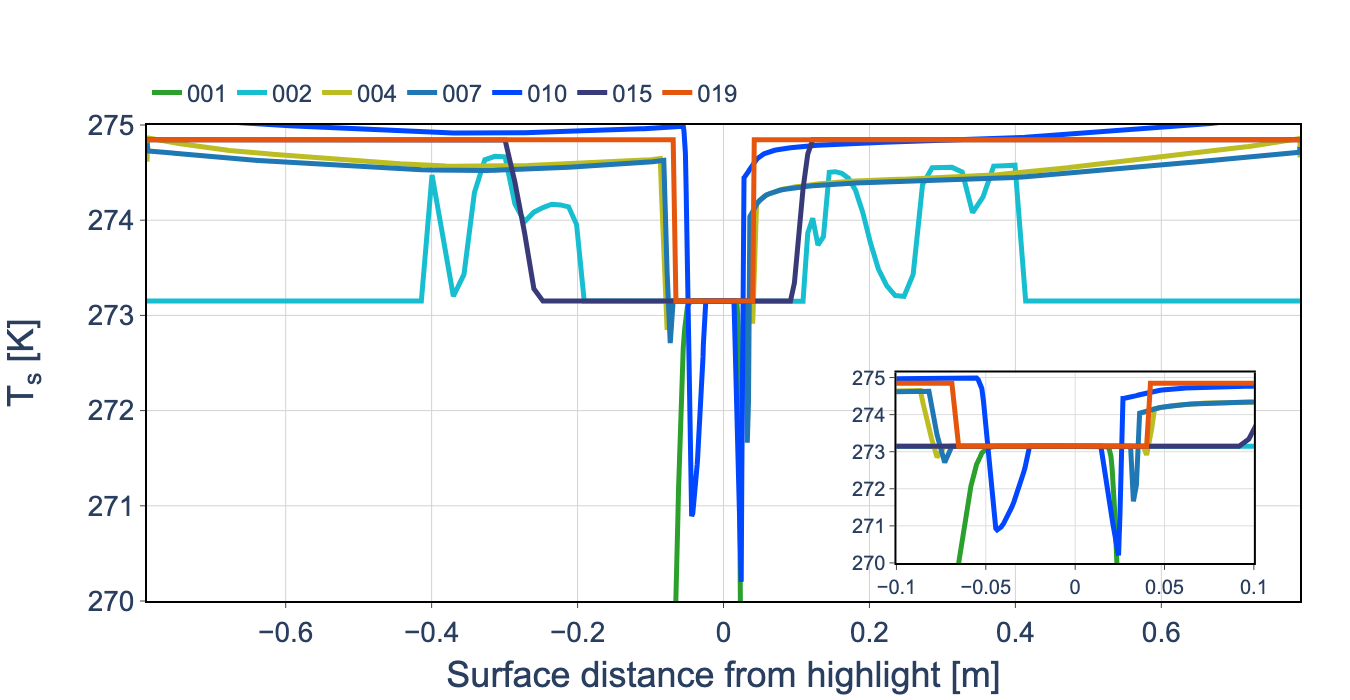
\includegraphics[width=0.5\textwidth]{FIGURES/SURF_TEMP_FF/tc_oneram6_L1_surface_temperature_vs_s_slice_0p75_roughness_1mm.png}

\vspace{0.05cm}

\textbf{$y=0.75$ m }
}

% ------------------------------------------------------------
% Inboard and outboard slices
% ------------------------------------------------------------
\only<2>{
\begin{columns}[T,onlytextwidth]

\begin{column}{0.50\textwidth}
    \centering
    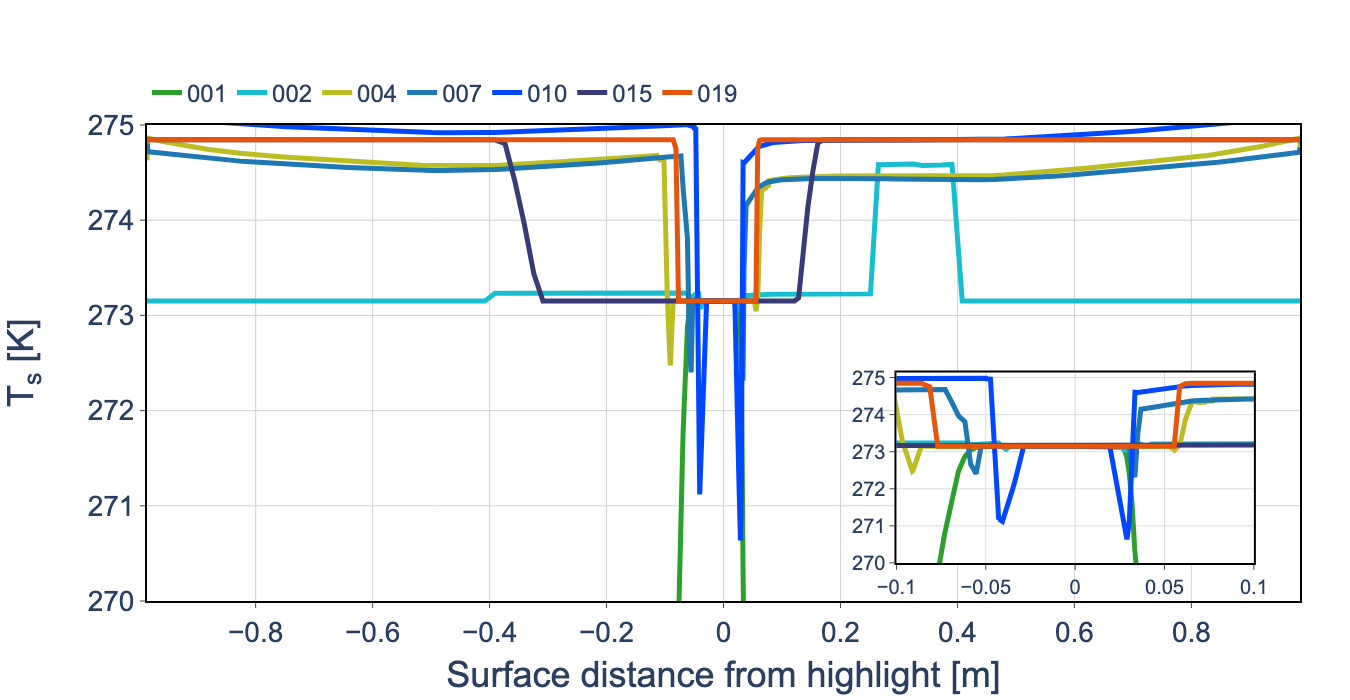
\includegraphics[width=0.94\textwidth]{FIGURES/SURF_TEMP_FF/tc_oneram6_L1_surface_temperature_vs_s_slice_0p1_roughness_1mm.png}

    \vspace{0.05cm}

    \textbf{$y=0.10$ m}
\end{column}

\begin{column}{0.50\textwidth}
    \centering
    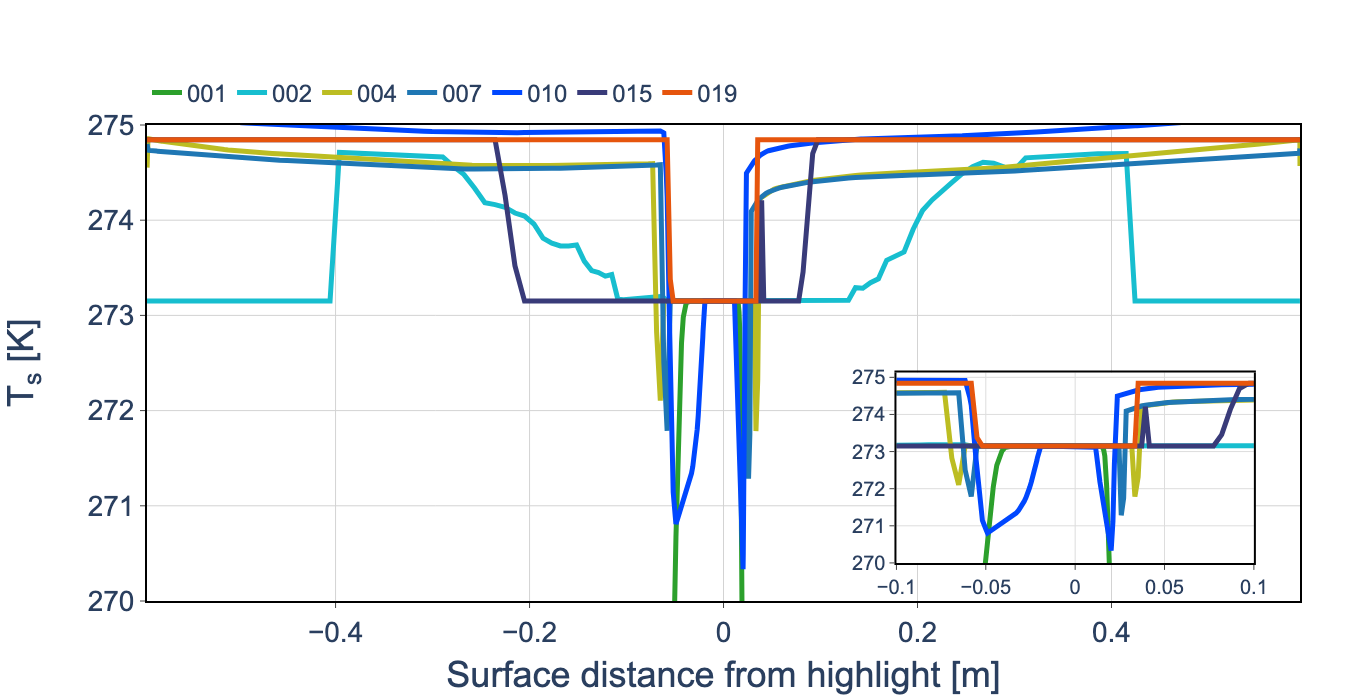
\includegraphics[width=0.94\textwidth]{FIGURES/SURF_TEMP_FF/tc_oneram6_L1_surface_temperature_vs_s_slice_1p4_roughness_1mm.png}

    \vspace{0.05cm}

    \textbf{$y=1.40$ m}
\end{column}

\end{columns}
}

\vspace{0.10cm}

\begin{block}{\scriptsize Observations}
\begin{itemize}
    \item<1-> Most submissions predict surface temperatures close to the freezing temperature over a large portion of the surface.
    \item<1-> Local code-to-code differences are concentrated near the leading edge.
    \item<2-> Similar differences are observed at the inboard and outboard spanwise stations.
\end{itemize}
\end{block}

\end{frame}


% ============================================================
% ONERA M6 -- Mean Surface Temperature
% ============================================================

\begin{frame}{\small ONERA M6 -- Mean Surface Temperature Grid Convergence}
\scriptsize

% ------------------------------------------------------------
% Middle slice -- 1 mm roughness
% ------------------------------------------------------------
\only<1>{
\begin{columns}[T,onlytextwidth]

\begin{column}{0.50\textwidth}
    \centering
    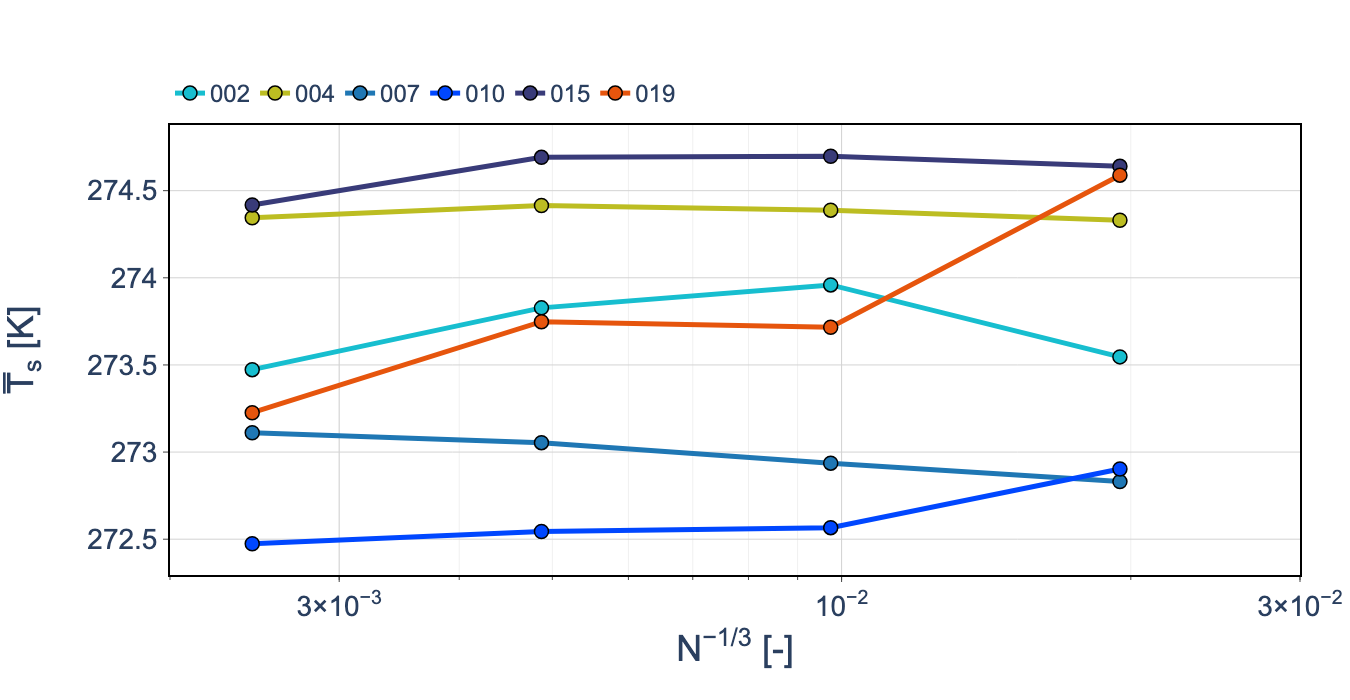
\includegraphics[width=0.94\textwidth]{FIGURES/SURF_TEMP_FF/tc_oneram6_mean_surface_temperature_vs_n_slice_0p75_roughness_1mm.png}

    \vspace{0.05cm}
\end{column}

\begin{column}{0.50\textwidth}
    \centering
    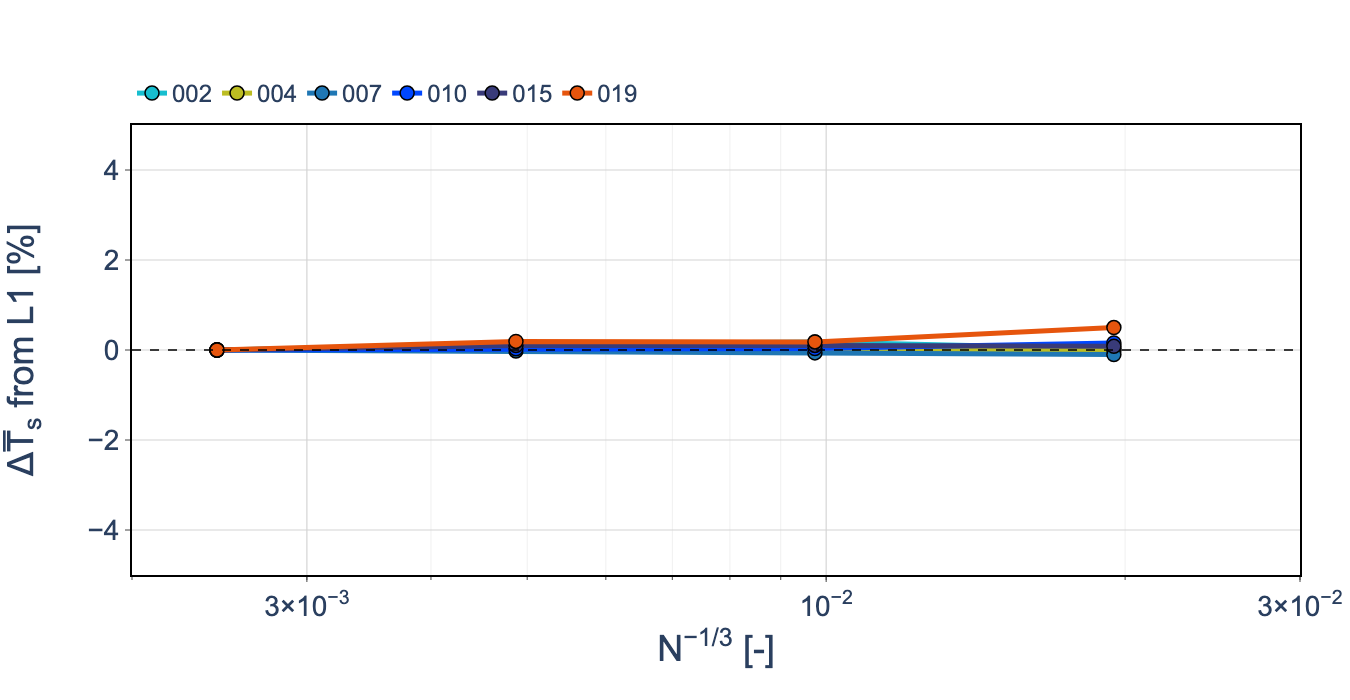
\includegraphics[width=0.94\textwidth]{FIGURES/SURF_TEMP_FF/tc_oneram6_mean_surface_temperature_vs_n_slice_0p75_roughness_1mm_relative_to_l1.png}

    \vspace{0.05cm}

\end{column}

\end{columns}

\vspace{0.05cm}

\centering
\textbf{$y=0.75$ m}
}

% ------------------------------------------------------------
% Inboard and outboard slices -- 1 mm roughness
% ------------------------------------------------------------
\only<2>{
\begin{columns}[T,onlytextwidth]

\begin{column}{0.50\textwidth}
    \centering
    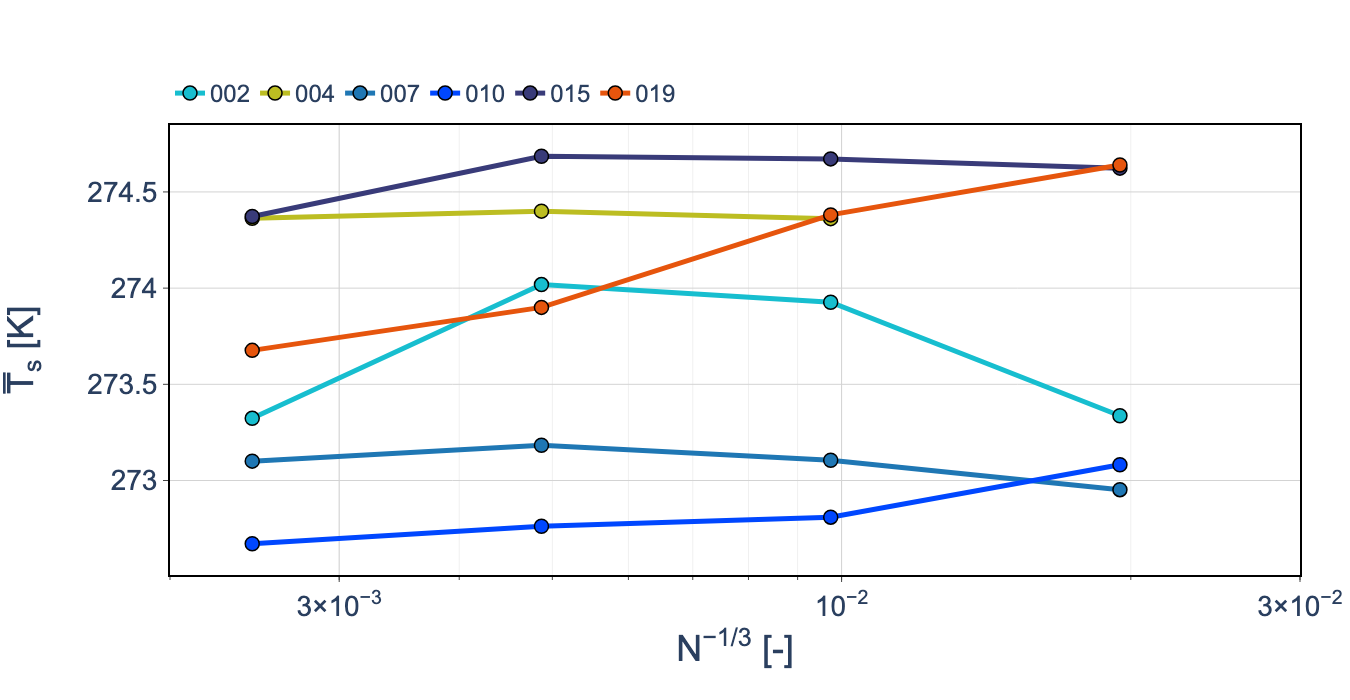
\includegraphics[width=0.94\textwidth]{FIGURES/SURF_TEMP_FF/tc_oneram6_mean_surface_temperature_vs_n_slice_0p1_roughness_1mm.png}

    \vspace{0.05cm}

    \textbf{$y=0.10$ m}
\end{column}

\begin{column}{0.50\textwidth}
    \centering
    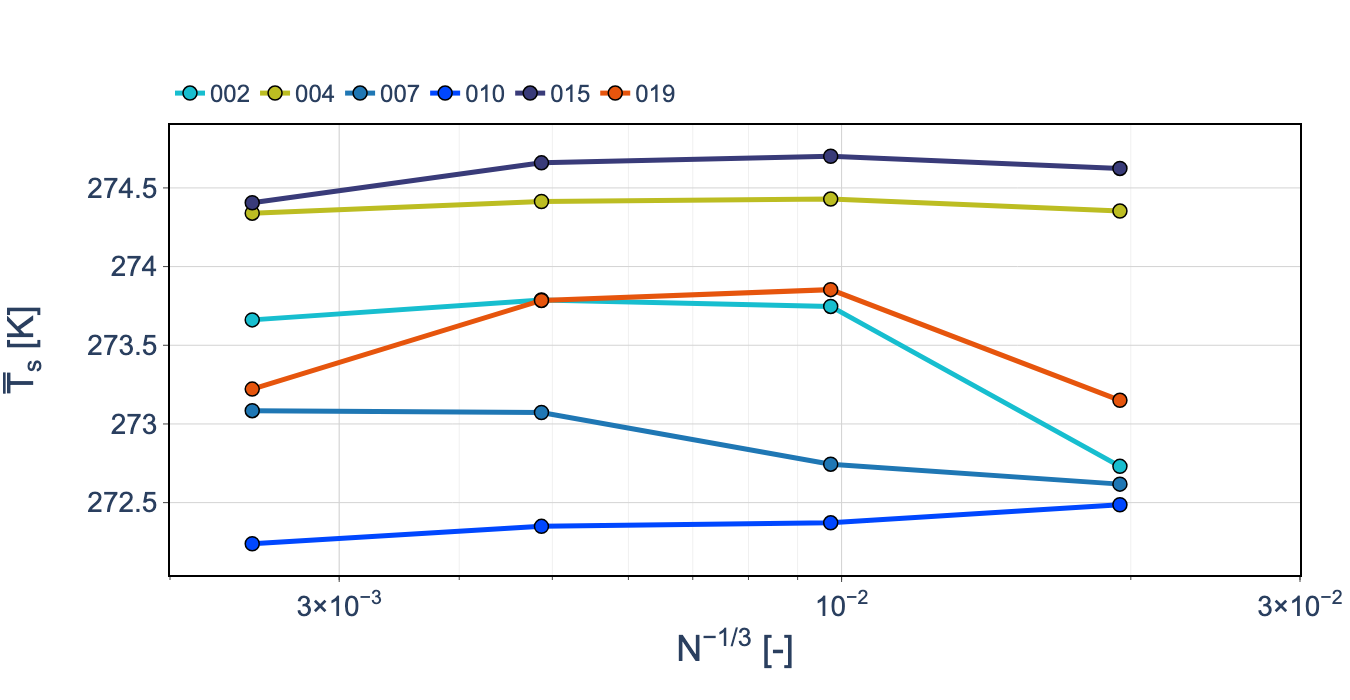
\includegraphics[width=0.94\textwidth]{FIGURES/SURF_TEMP_FF/tc_oneram6_mean_surface_temperature_vs_n_slice_1p4_roughness_1mm.png}

    \vspace{0.05cm}

    \textbf{$y=1.40$ m}
\end{column}

\end{columns}
}

% ------------------------------------------------------------
% Middle slice -- roughness sensitivity
% ------------------------------------------------------------
\only<3>{
\centering
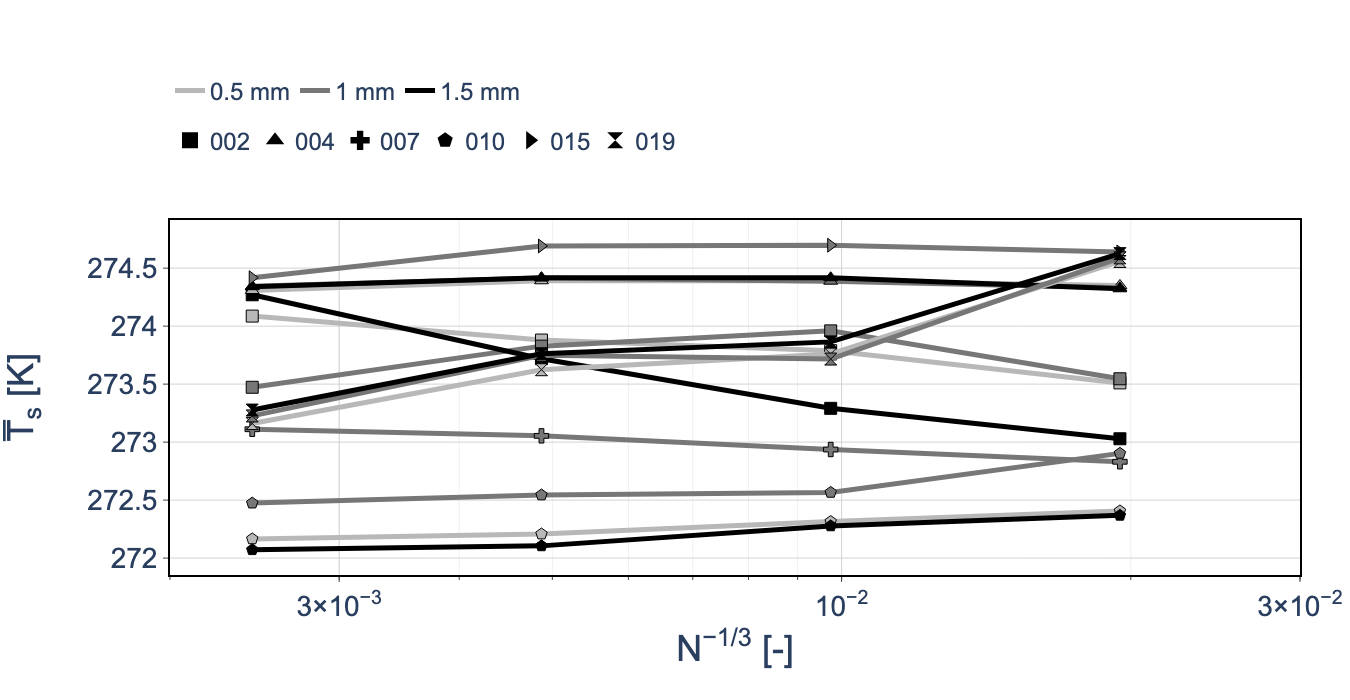
\includegraphics[width=0.5\textwidth]{FIGURES/SURF_TEMP_FF/tc_oneram6_mean_surface_temperature_vs_n_slice_0p75_grouped_roughness.png}

\vspace{0.05cm}

\textbf{$y=0.75$ m}
}

\vspace{0.10cm}

\begin{block}{\scriptsize Observations}
\begin{itemize}
    \item<1-> Mean $T_s$ is area-weighted ($ds$) over the iced surface ($h_{\mathrm{ice}}>0$).
    \item<1-> Grid sensitivity is limited ($<1\%$ for most submissions), with closely clustered predictions.
    \item<2-> Similar behavior is observed across the spanwise stations.
    \item<3-> Roughness changes mean $T_s$ by approximately $\pm1$ K, with a code-dependent response.
\end{itemize}
\end{block}

\end{frame}

% ============================================================
% ONERA M6 -- Participant-Level Roughness Sensitivity
% ============================================================

\begin{frame}{\small ONERA M6 -- Participant-Level Mean Surface Temperature Roughness Sensitivity (L1)}
\scriptsize
\vspace{-0.2cm}
\centering
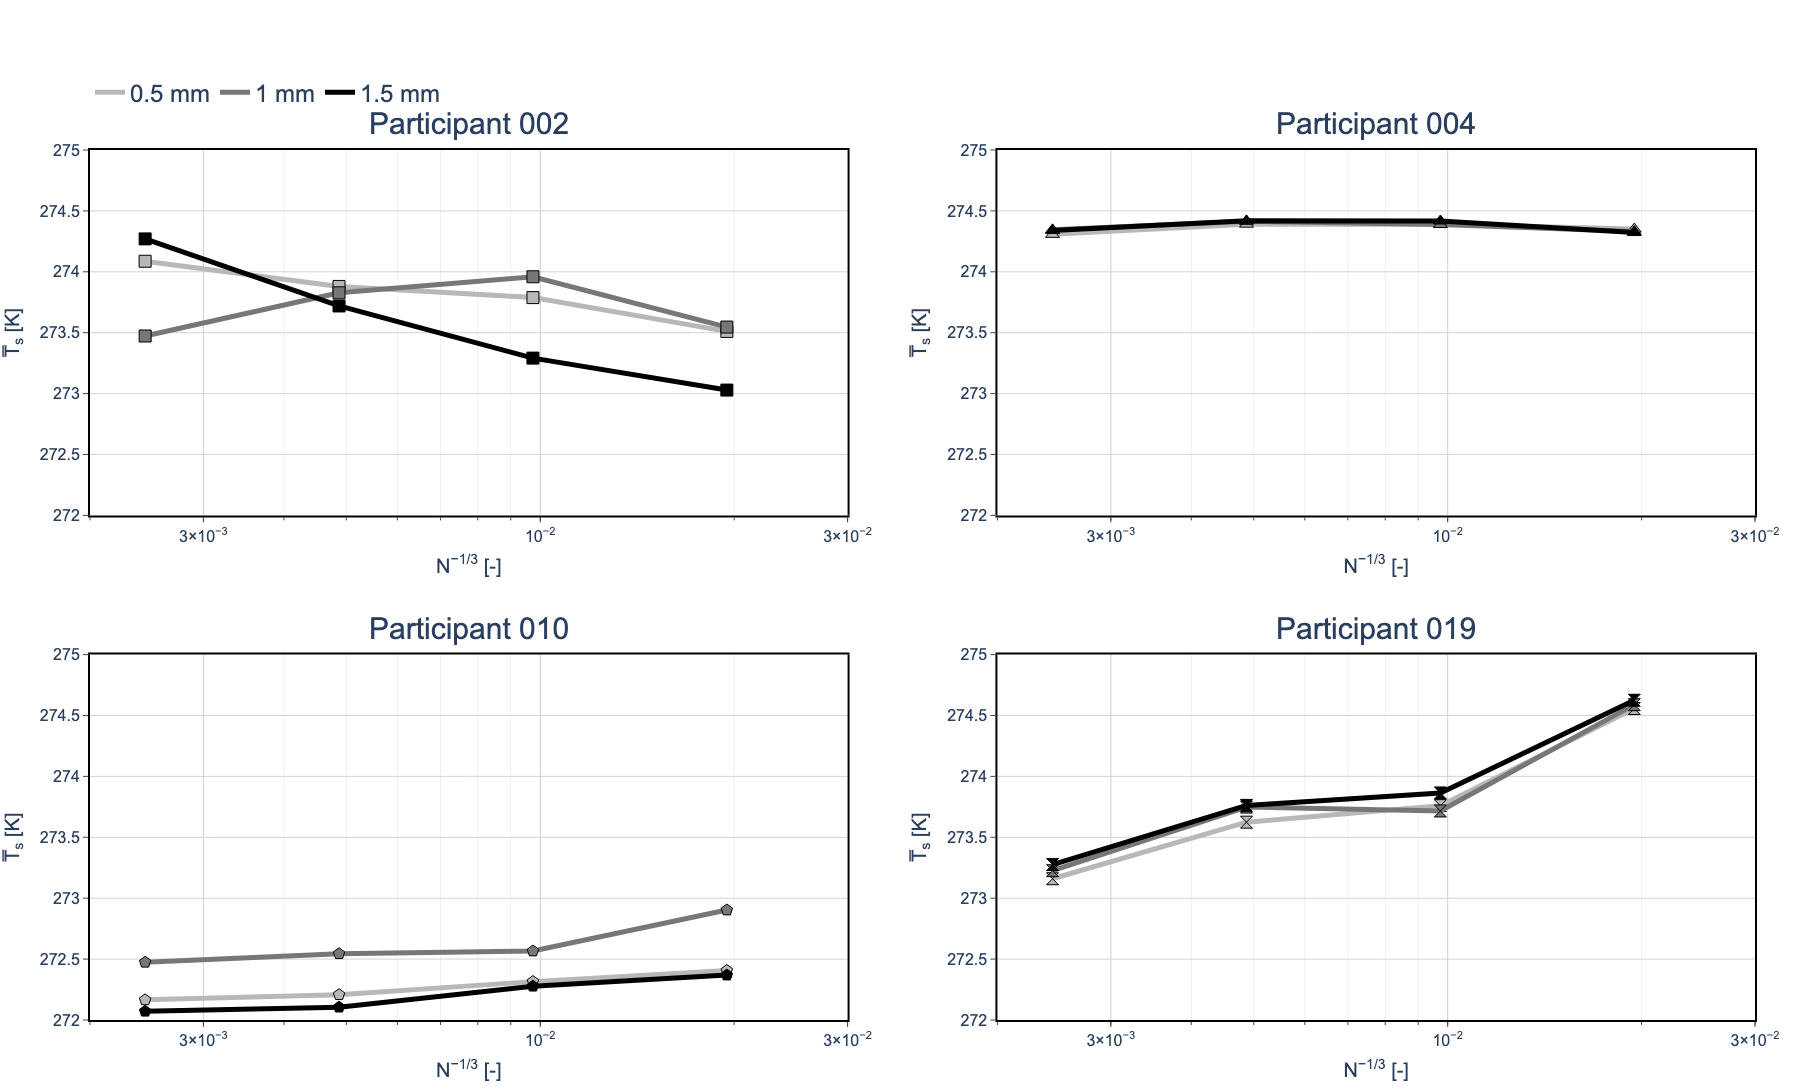
\includegraphics[width=0.8\textwidth]{FIGURES/SURF_TEMP_FF/tc_oneram6_mean_surface_temperature_vs_n_slice_0p75_grouped_roughness_participants.png}

\end{frame}

% ============================================================
% ONERA M6 -- Integrated Convective Heat Transfer
% ============================================================

\begin{frame}[shrink=15]{\small ONERA M6 -- Integrated Convective Heat Transfer}
\scriptsize

\centering

\begin{minipage}{0.90\textwidth}
\begin{block}{\scriptsize Grid-Convergence Metric}
To assess whether the differences in the local $HTC$ distributions translate
into a clear grid-convergence behavior, an integrated convective heat-transfer
quantity is evaluated along the surface slice:
\[
\boxed{
Q_c'
=
\int
HTC(s)
\left[
T_s(s)-T_{\mathrm{rec}}(s)
\right]\,ds
}
\qquad
[Q_c'] = \mathrm{W/m}.
\]

The submitted $HTC$ and surface temperature $T_s$ are used directly.
The recovery temperature $T_{\mathrm{rec}}$, however, was not part of the
submitted dataset and must therefore be reconstructed.
\end{block}
\end{minipage}

\vspace{0.15cm}

\begin{minipage}{0.90\textwidth}
\begin{block}{\scriptsize Recovery Temperature Reconstruction}
The submitted pressure coefficient is used to estimate the local external-flow
state and subsequently the recovery temperature:
\[
\boxed{
C_p(s)
\;\longrightarrow\;
p_e(s)
\;\longrightarrow\;
M_e(s)
\;\longrightarrow\;
T_e(s)
\;\longrightarrow\;
T_{\mathrm{rec}}(s)
}
\]

Assuming $p_s \simeq p_e$ and an isentropic external flow,
\[
\frac{p_e}{p_\infty}
=
1+\frac{\gamma}{2}M_\infty^2 C_{p,e},
\qquad
M_e^2
=
\frac{2}{\gamma-1}
\left[
\left(\frac{p_0}{p_e}\right)^{(\gamma-1)/\gamma}-1
\right],
\]
\[
T_e
=
\frac{T_0}
{1+\dfrac{\gamma-1}{2}M_e^2},
\qquad
T_{\mathrm{rec}}
=
T_e
\left[
1+r\frac{\gamma-1}{2}M_e^2
\right],
\qquad
r=Pr^{1/3}\approx0.9.
\]

\end{block}
\end{minipage}

\end{frame}

% ============================================================
% ONERA M6 -- Recovery Temperature Distribution
% ============================================================

\begin{frame}{\small ONERA M6 -- Reconstructed Recovery Temperature Distribution (L1)}
\scriptsize

% ------------------------------------------------------------
% Middle slice
% ------------------------------------------------------------
\only<1>{
\centering
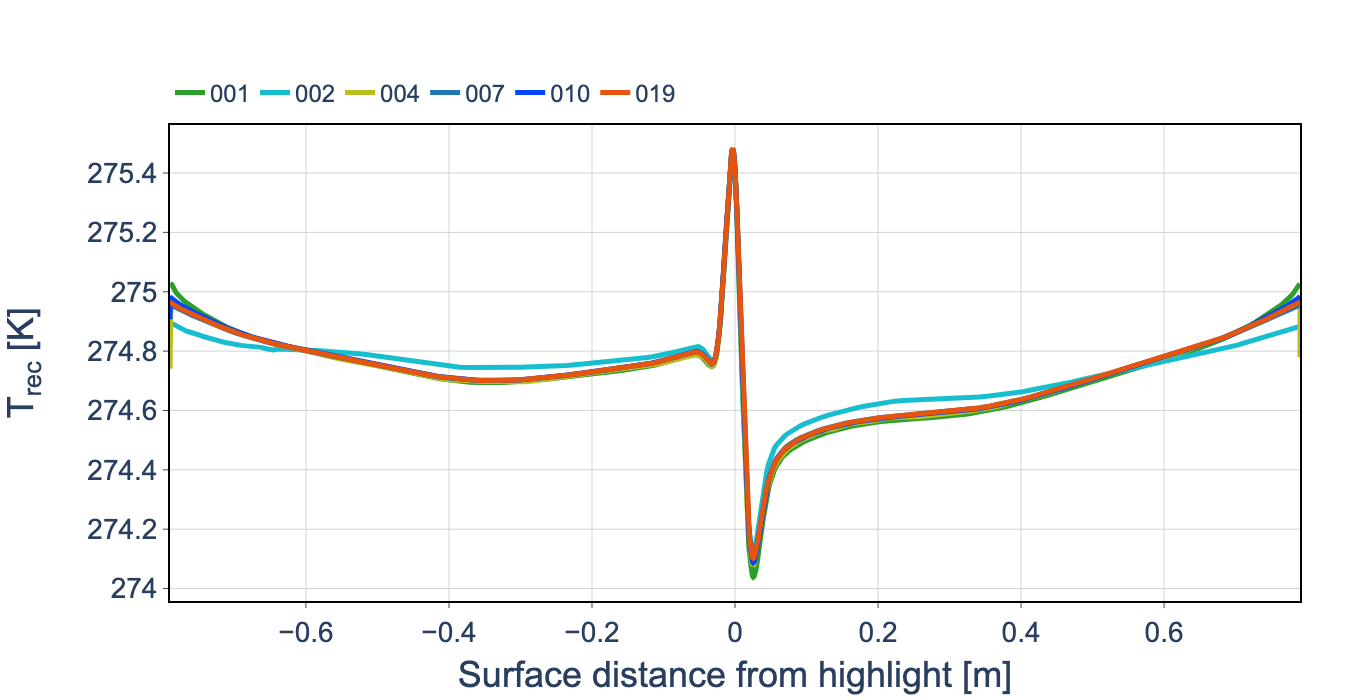
\includegraphics[width=0.5\textwidth]{FIGURES/HTC/tc_oneram6_L1_recovery_temperature_vs_s_slice_0p75_roughness_1mm.png}

\vspace{0.05cm}

\textbf{$y=0.75$ m}
}

% ------------------------------------------------------------
% Inboard and outboard slices
% ------------------------------------------------------------
\only<2>{
\begin{columns}[T,onlytextwidth]

\begin{column}{0.50\textwidth}
    \centering
    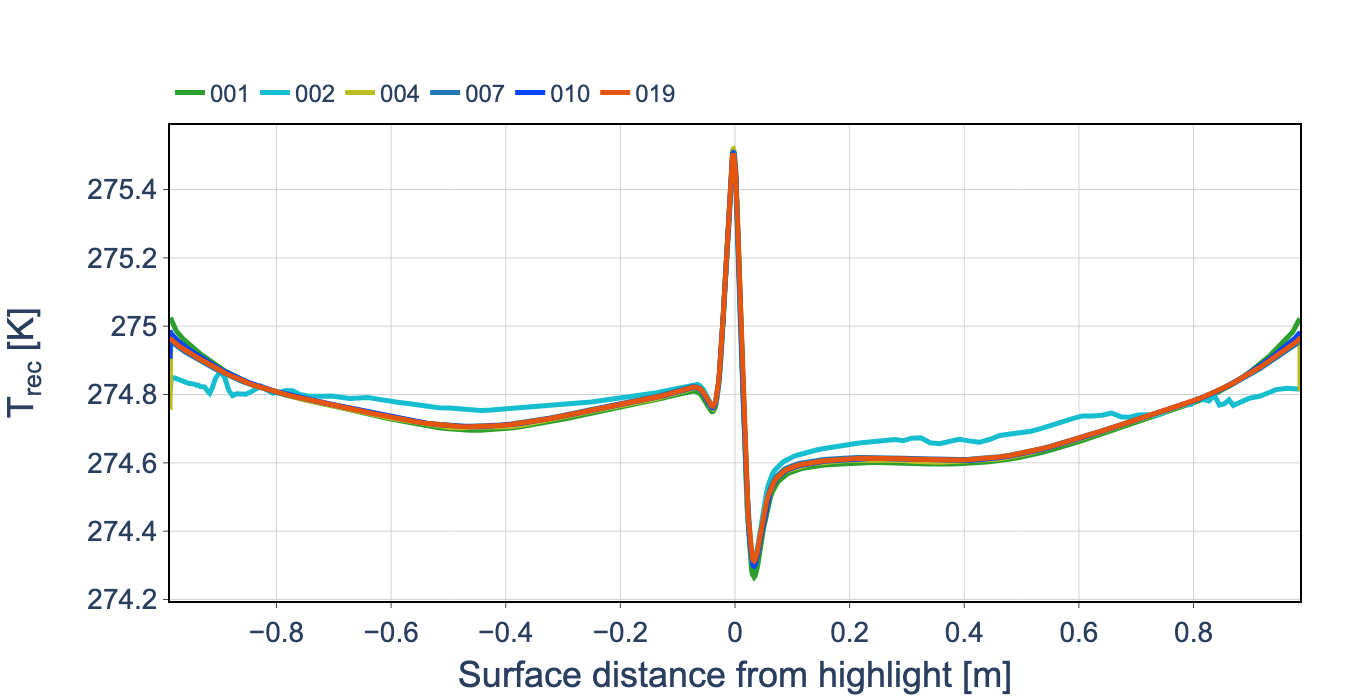
\includegraphics[width=0.92\textwidth]{FIGURES/HTC/tc_oneram6_L1_recovery_temperature_vs_s_slice_0p1_roughness_1mm.png}

    \vspace{0.05cm}

    \textbf{$y=0.10$ m}
\end{column}

\begin{column}{0.50\textwidth}
    \centering
    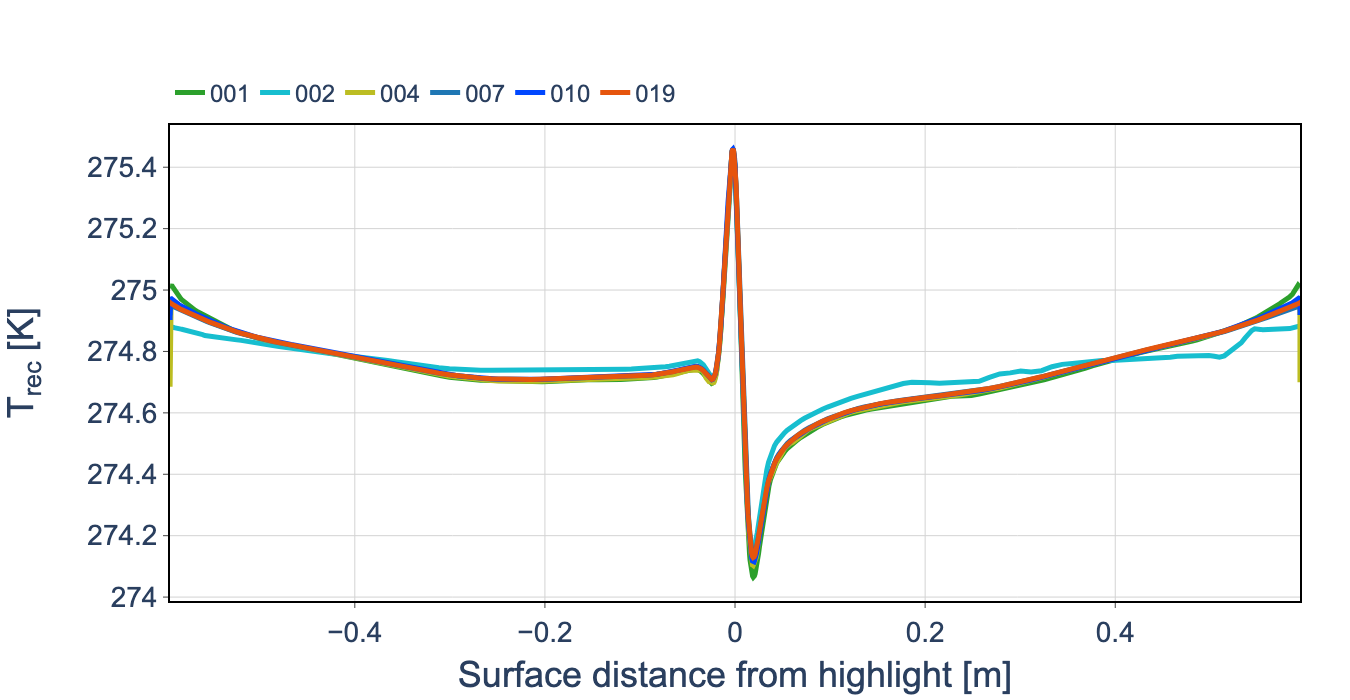
\includegraphics[width=0.92\textwidth]{FIGURES/HTC/tc_oneram6_L1_recovery_temperature_vs_s_slice_1p4_roughness_1mm.png}

    \vspace{0.05cm}

    \textbf{$y=1.40$ m}
\end{column}

\end{columns}
}

\vspace{0.05cm}

\begin{block}{\scriptsize Observations}
\begin{itemize}
    \item<1-> The reconstructed recovery-temperature distributions are closely aligned across submissions.
    \item<1-> This agreement is consistent with the good code-to-code agreement previously observed for $C_p$, from which $T_{\mathrm{rec}}$ is reconstructed.
    \item<2-> Similar agreement is observed at the inboard and outboard spanwise stations.
\end{itemize}
\end{block}

\end{frame}

% ============================================================
% ONERA M6 -- Convective Heat Transfer Grid Convergence
% ============================================================

\begin{frame}{\small ONERA M6 -- Convective Heat Transfer Grid Convergence}
\scriptsize

% ------------------------------------------------------------
% Middle slice -- absolute and relative to L1
% ------------------------------------------------------------
\only<1>{
\begin{columns}[T,onlytextwidth]

\begin{column}{0.50\textwidth}
    \centering
    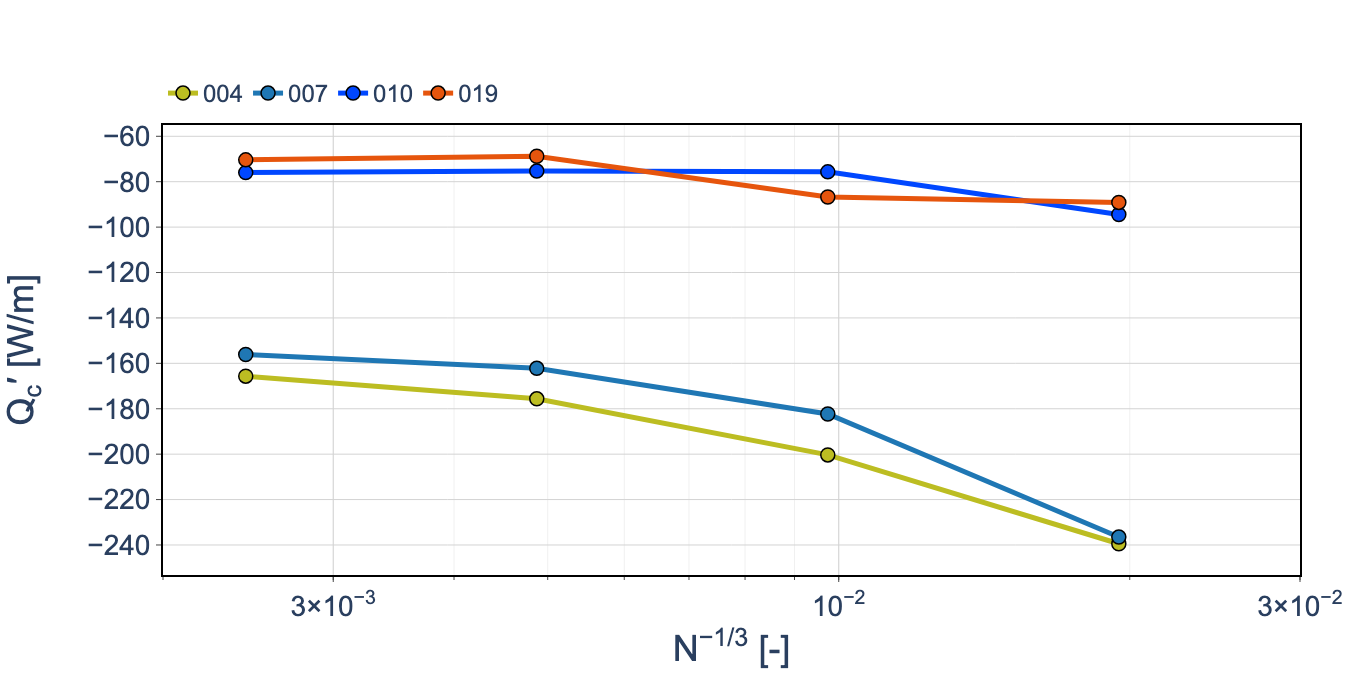
\includegraphics[width=0.94\textwidth]{FIGURES/HTC/tc_oneram6_qc_prime_vs_n_y_0.75.png}
\end{column}

\begin{column}{0.50\textwidth}
    \centering
    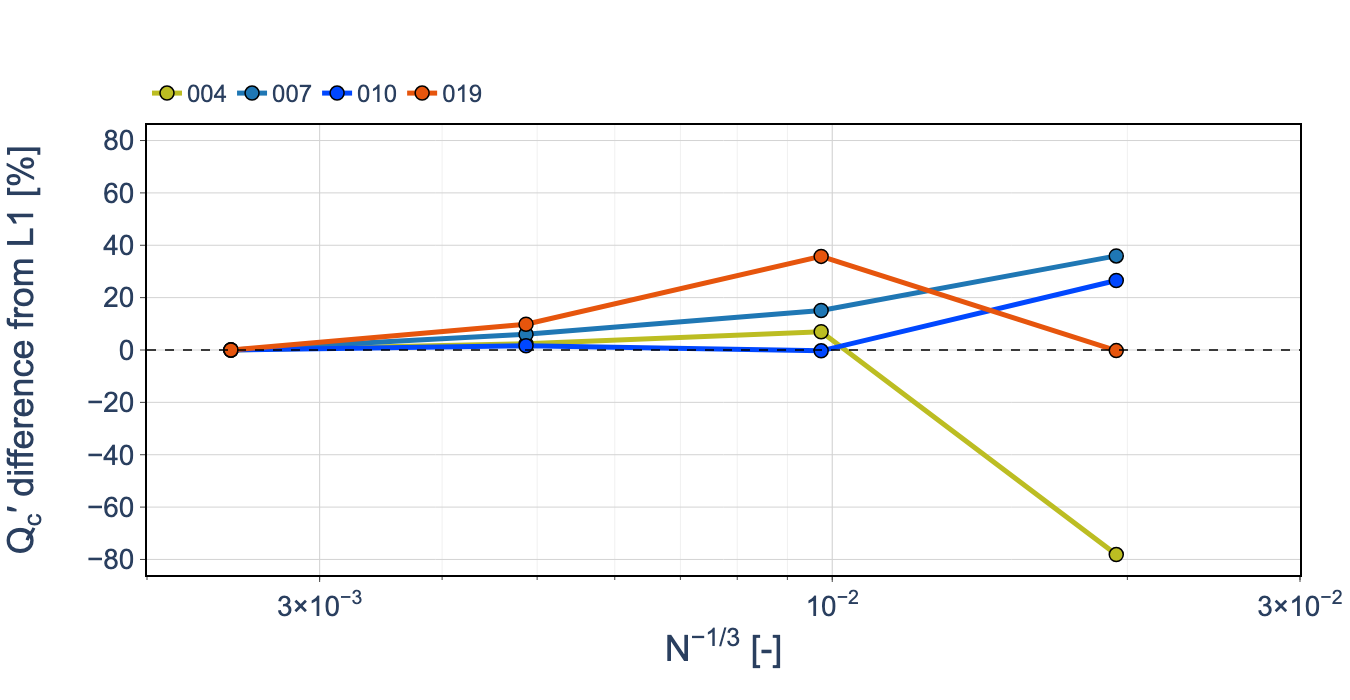
\includegraphics[width=0.94\textwidth]{FIGURES/HTC/tc_oneram6_qc_prime_vs_n_y_0.1_relative_to_l1.png}
\end{column}

\end{columns}

\vspace{0.05cm}

\centering
\textbf{$y=0.75$ m}
}

% ------------------------------------------------------------
% Inboard and outboard slices -- 1 mm roughness
% ------------------------------------------------------------
\only<2>{
\begin{columns}[T,onlytextwidth]

\begin{column}{0.50\textwidth}
    \centering
    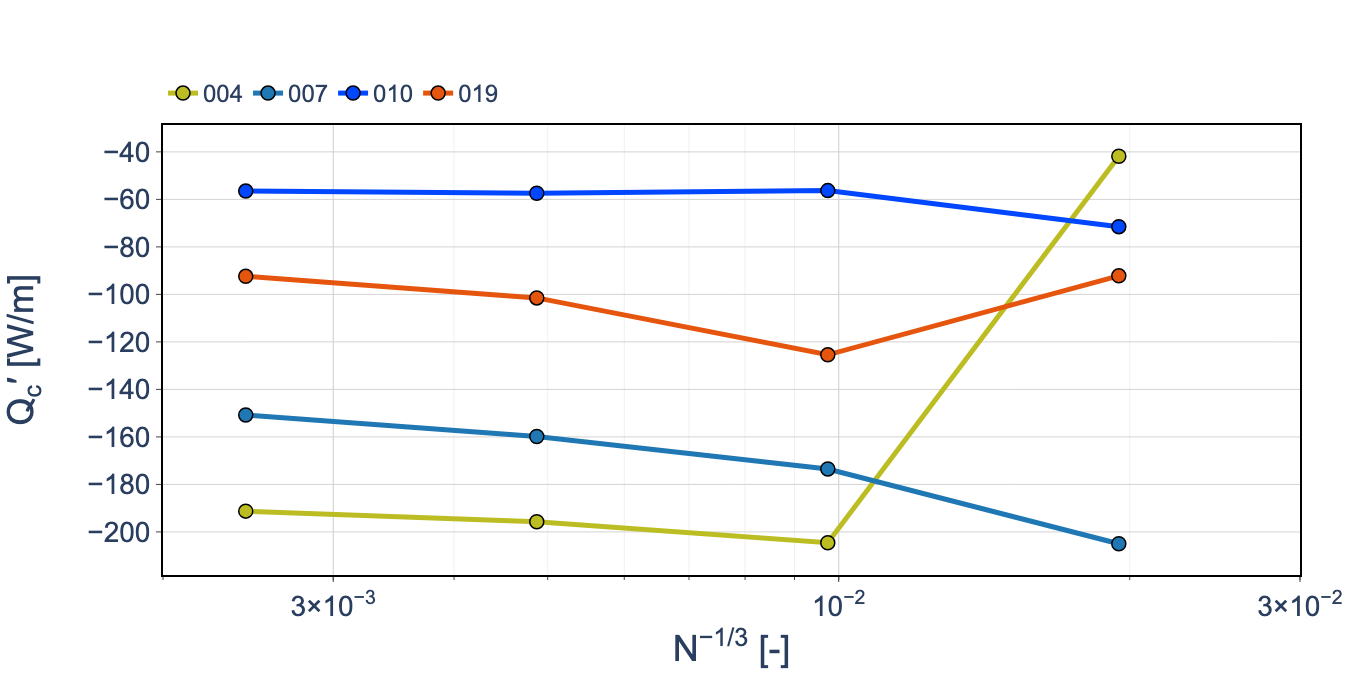
\includegraphics[width=0.94\textwidth]{FIGURES/HTC/tc_oneram6_qc_prime_vs_n_y_0.1.png}

    \vspace{0.05cm}

    \textbf{$y=0.10$ m}
\end{column}

\begin{column}{0.50\textwidth}
    \centering
    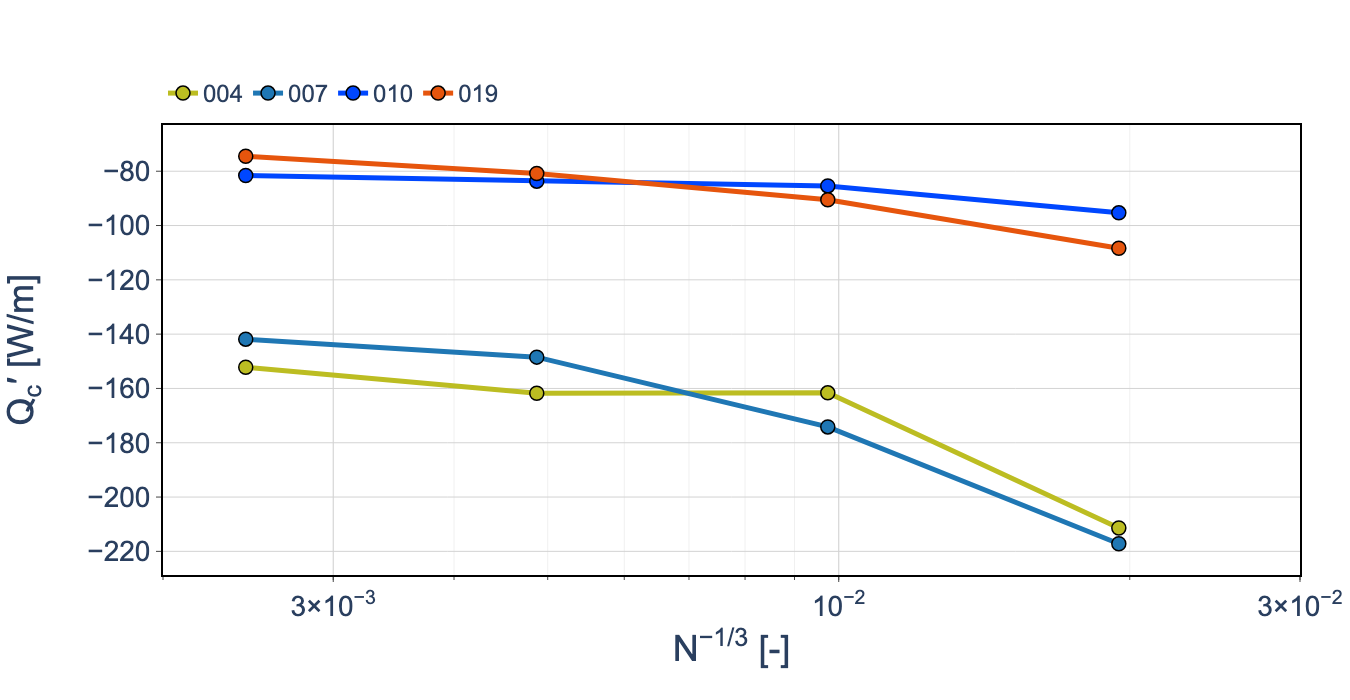
\includegraphics[width=0.94\textwidth]{FIGURES/HTC/tc_oneram6_qc_prime_vs_n_y_1.4.png}

    \vspace{0.05cm}

    \textbf{$y=1.40$ m}
\end{column}

\end{columns}
}

% ------------------------------------------------------------
% Middle slice -- roughness sensitivity
% ------------------------------------------------------------
\only<3>{
\centering
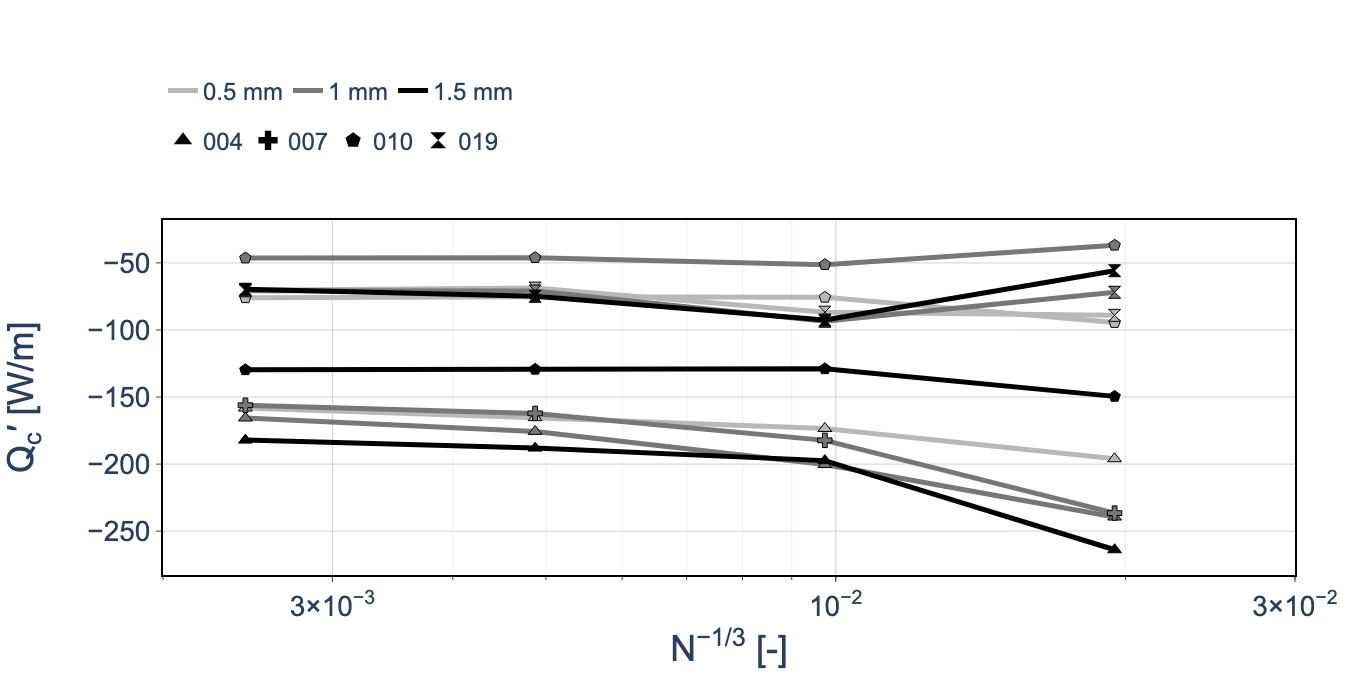
\includegraphics[width=0.5\textwidth]{FIGURES/HTC/tc_oneram6_qc_prime_vs_n_y_0.75_grouped_roughness.png}

\vspace{0.05cm}

\textbf{$y=0.75$ m- Roughness Sensitivity}
}

\vspace{0.10cm}

\begin{block}{\scriptsize Observations}
\begin{itemize}
    \item<1-> Considerable code-to-code variability is observed in $Q_c'$, exceeding the L1--L2 grid effect for most submissions.
    \item<2-> Large variability persists across all spanwise stations.
    \item<3-> Increasing surface roughness systematically increases $|Q_c'|$.
\end{itemize}
\end{block}

\end{frame}

% ============================================================
% ONERA M6 -- Participant-Level Roughness Sensitivity
% ============================================================

\begin{frame}{\small ONERA M6 -- Participant-Level HTC Roughness Sensitivity (L1)}
\scriptsize
\vspace{-0.2cm}
\centering
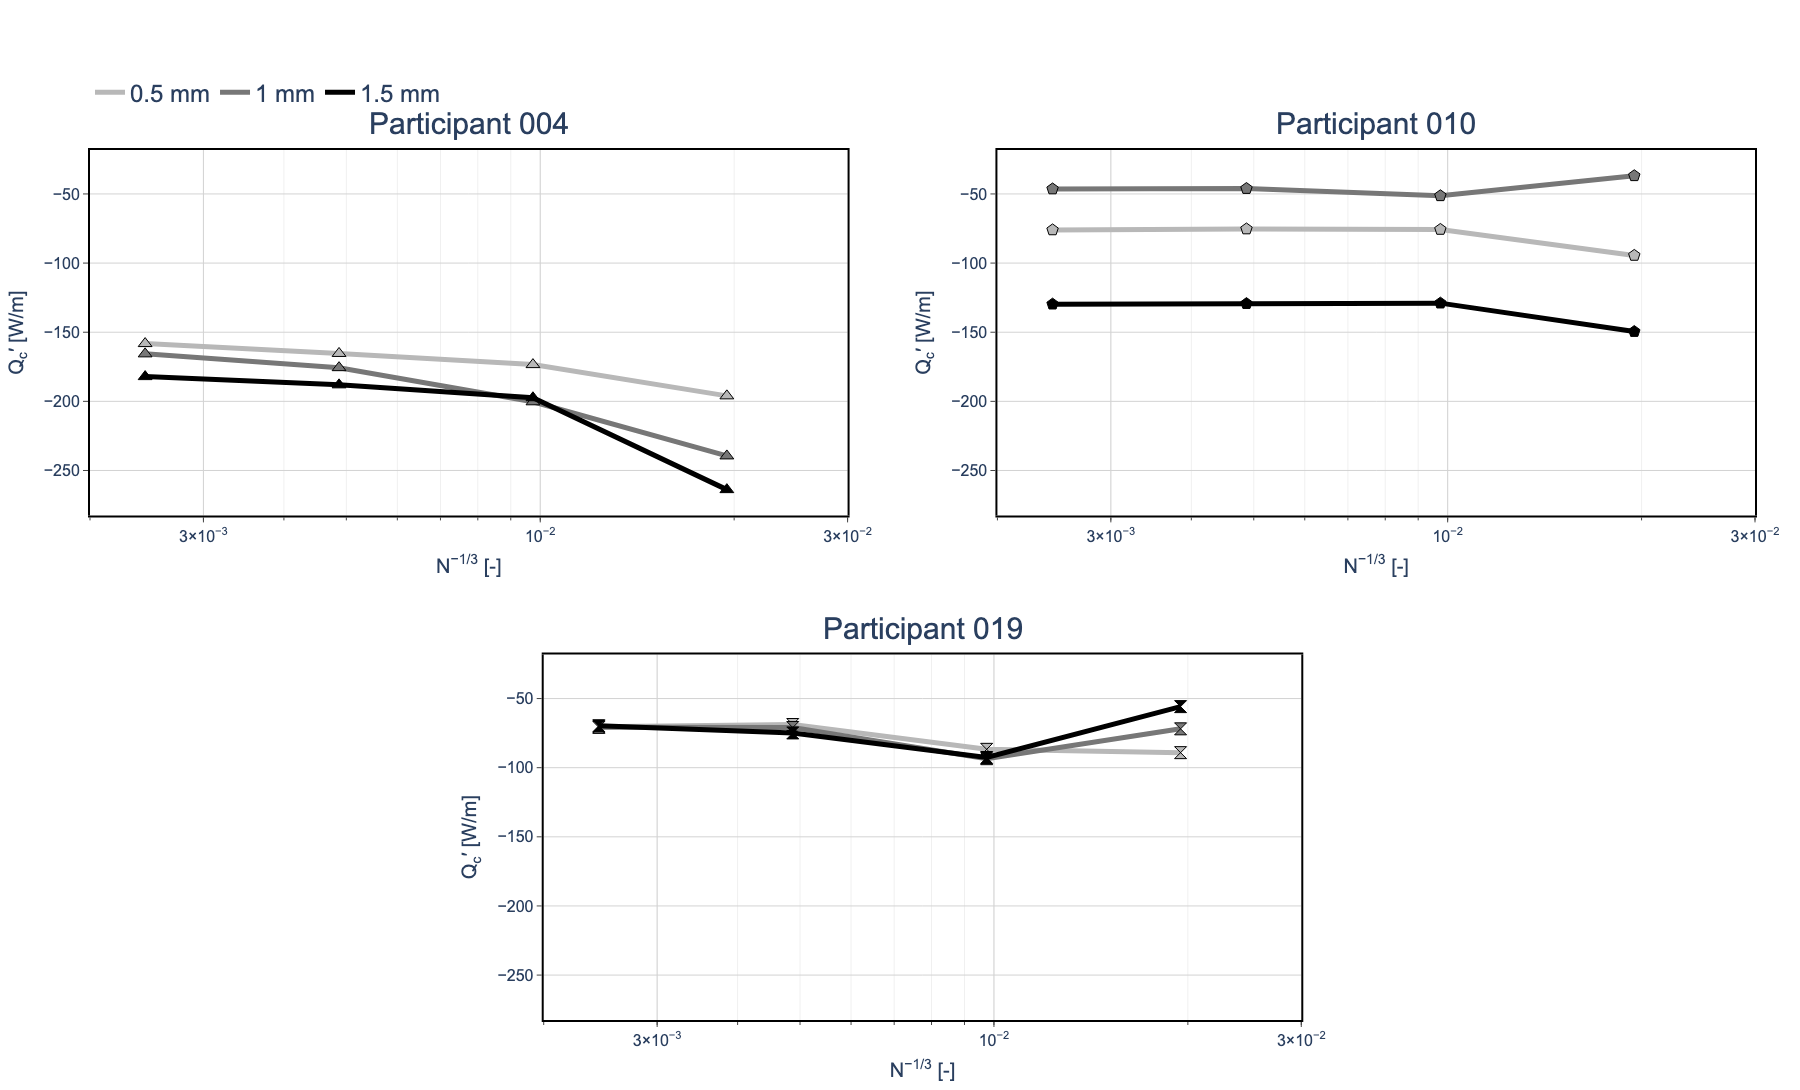
\includegraphics[width=0.8\textwidth]{FIGURES/HTC/tc_oneram6_qc_prime_vs_n_y_0.75_grouped_roughness_participants.png}

\end{frame}

% ============================================================
% ONERA M6 -- Freezing Fraction Distribution
% ============================================================

\begin{frame}{\small ONERA M6 -- Freezing-Fraction Distribution (L1)}
\scriptsize

% ------------------------------------------------------------
% Middle slice
% ------------------------------------------------------------
\only<1>{
\centering
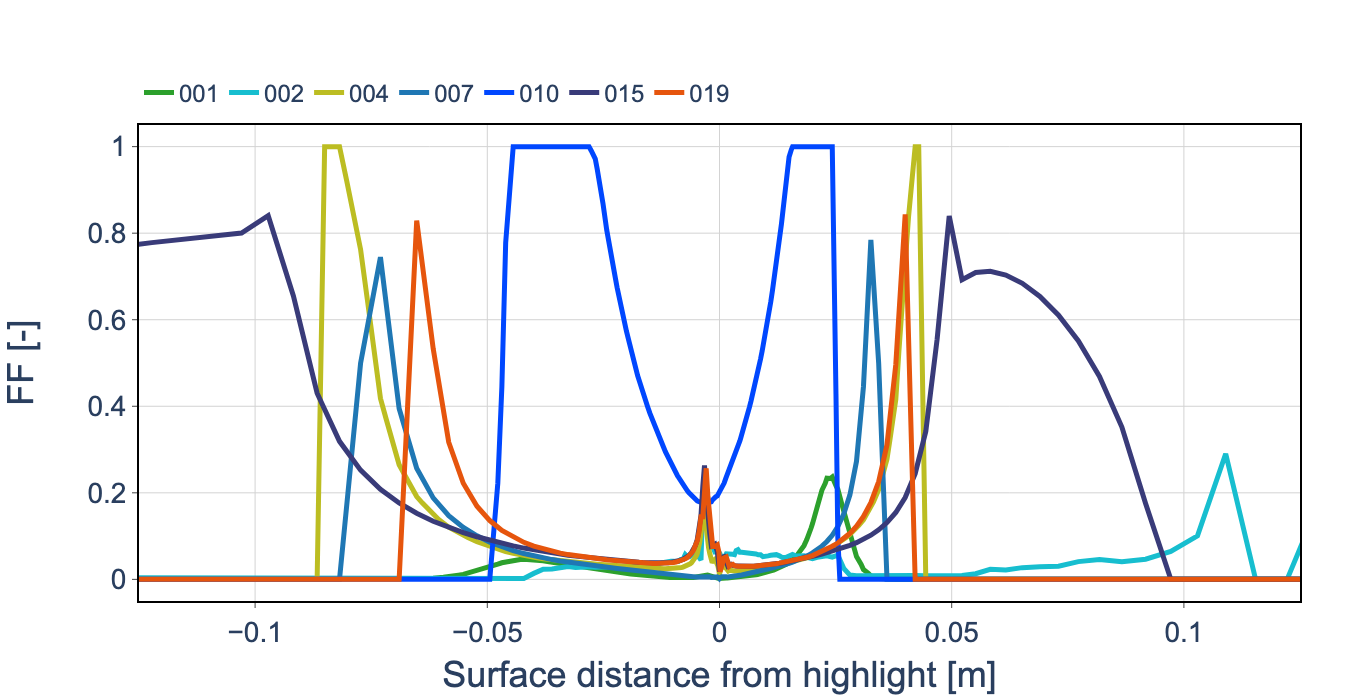
\includegraphics[width=0.5\textwidth]{FIGURES/SURF_TEMP_FF/tc_oneram6_L1_freezing_fraction_vs_s_slice_0p75_roughness_1mm.png}

\vspace{0.05cm}

\textbf{$y=0.75$ m}
}

% ------------------------------------------------------------
% Inboard and outboard slices
% ------------------------------------------------------------
\only<2>{
\begin{columns}[T,onlytextwidth]

\begin{column}{0.50\textwidth}
    \centering
    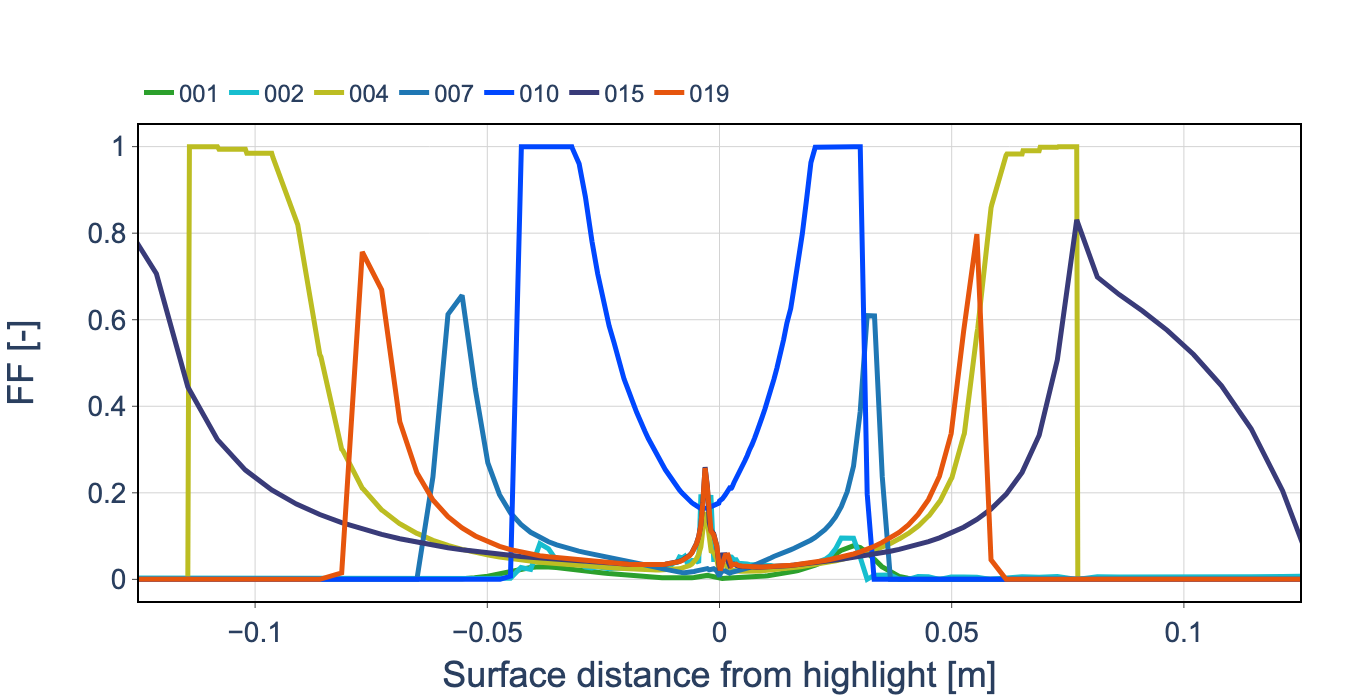
\includegraphics[width=0.94\textwidth]{FIGURES/SURF_TEMP_FF/tc_oneram6_L1_freezing_fraction_vs_s_slice_0p1_roughness_1mm.png}

    \vspace{0.05cm}

    \textbf{$y=0.10$ m}
\end{column}

\begin{column}{0.50\textwidth}
    \centering
    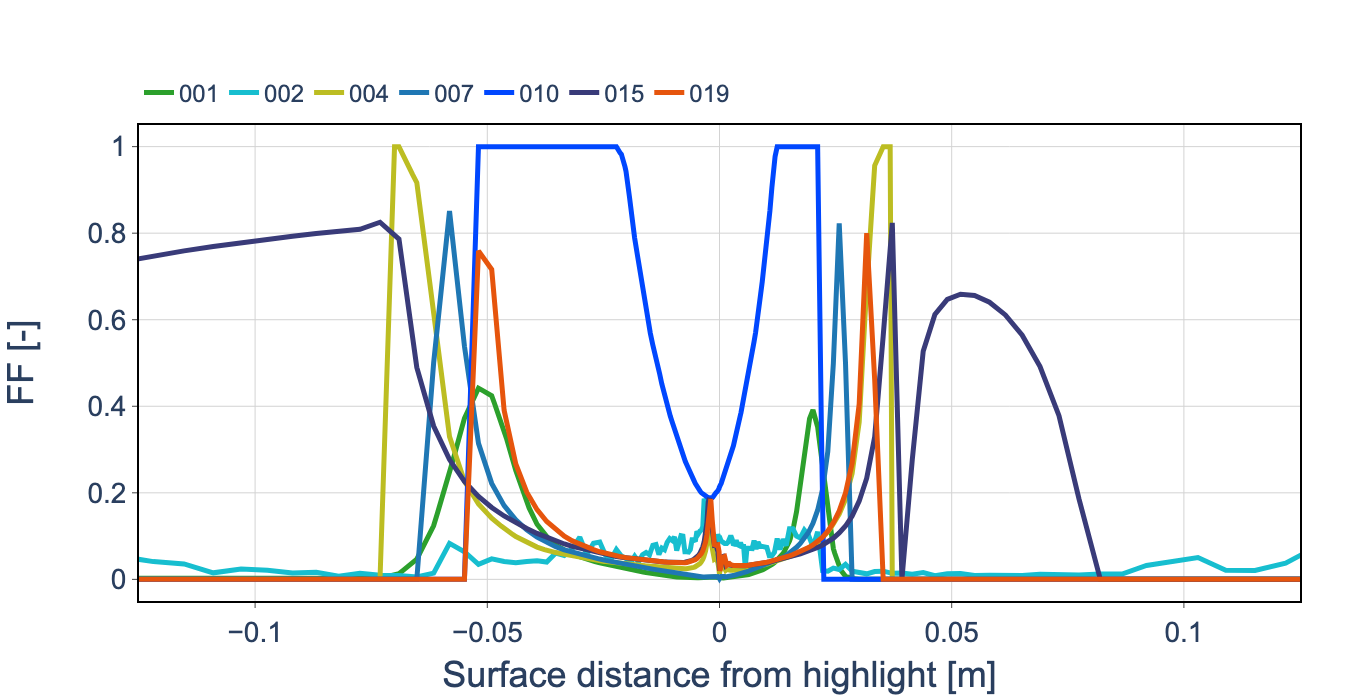
\includegraphics[width=0.94\textwidth]{FIGURES/SURF_TEMP_FF/tc_oneram6_L1_freezing_fraction_vs_s_slice_1p4_roughness_1mm.png}

    \vspace{0.05cm}

    \textbf{$y=1.40$ m}
\end{column}

\end{columns}
}

\vspace{0.10cm}

\begin{block}{\scriptsize Observations}
\begin{itemize}
    \item<1-> Large code-to-code differences are observed in both the magnitude and spatial extent of the predicted freezing fraction.
    \item<2-> Substantial differences in the predicted freezing regime persist across the inboard and outboard spanwise stations.
    \item<2-> Roughness affects the extent of the ice-covered region, with both the magnitude and direction of the response varying between codes.
\end{itemize}
\end{block}

\end{frame}

% ============================================================
% ONERA M6 -- Participant-Level Roughness Sensitivity
% ============================================================

\begin{frame}{\small ONERA M6 -- Participant-Level Freezing Fraction Roughness Sensitivity (L1)}
\scriptsize
\vspace{-0.2cm}
\centering
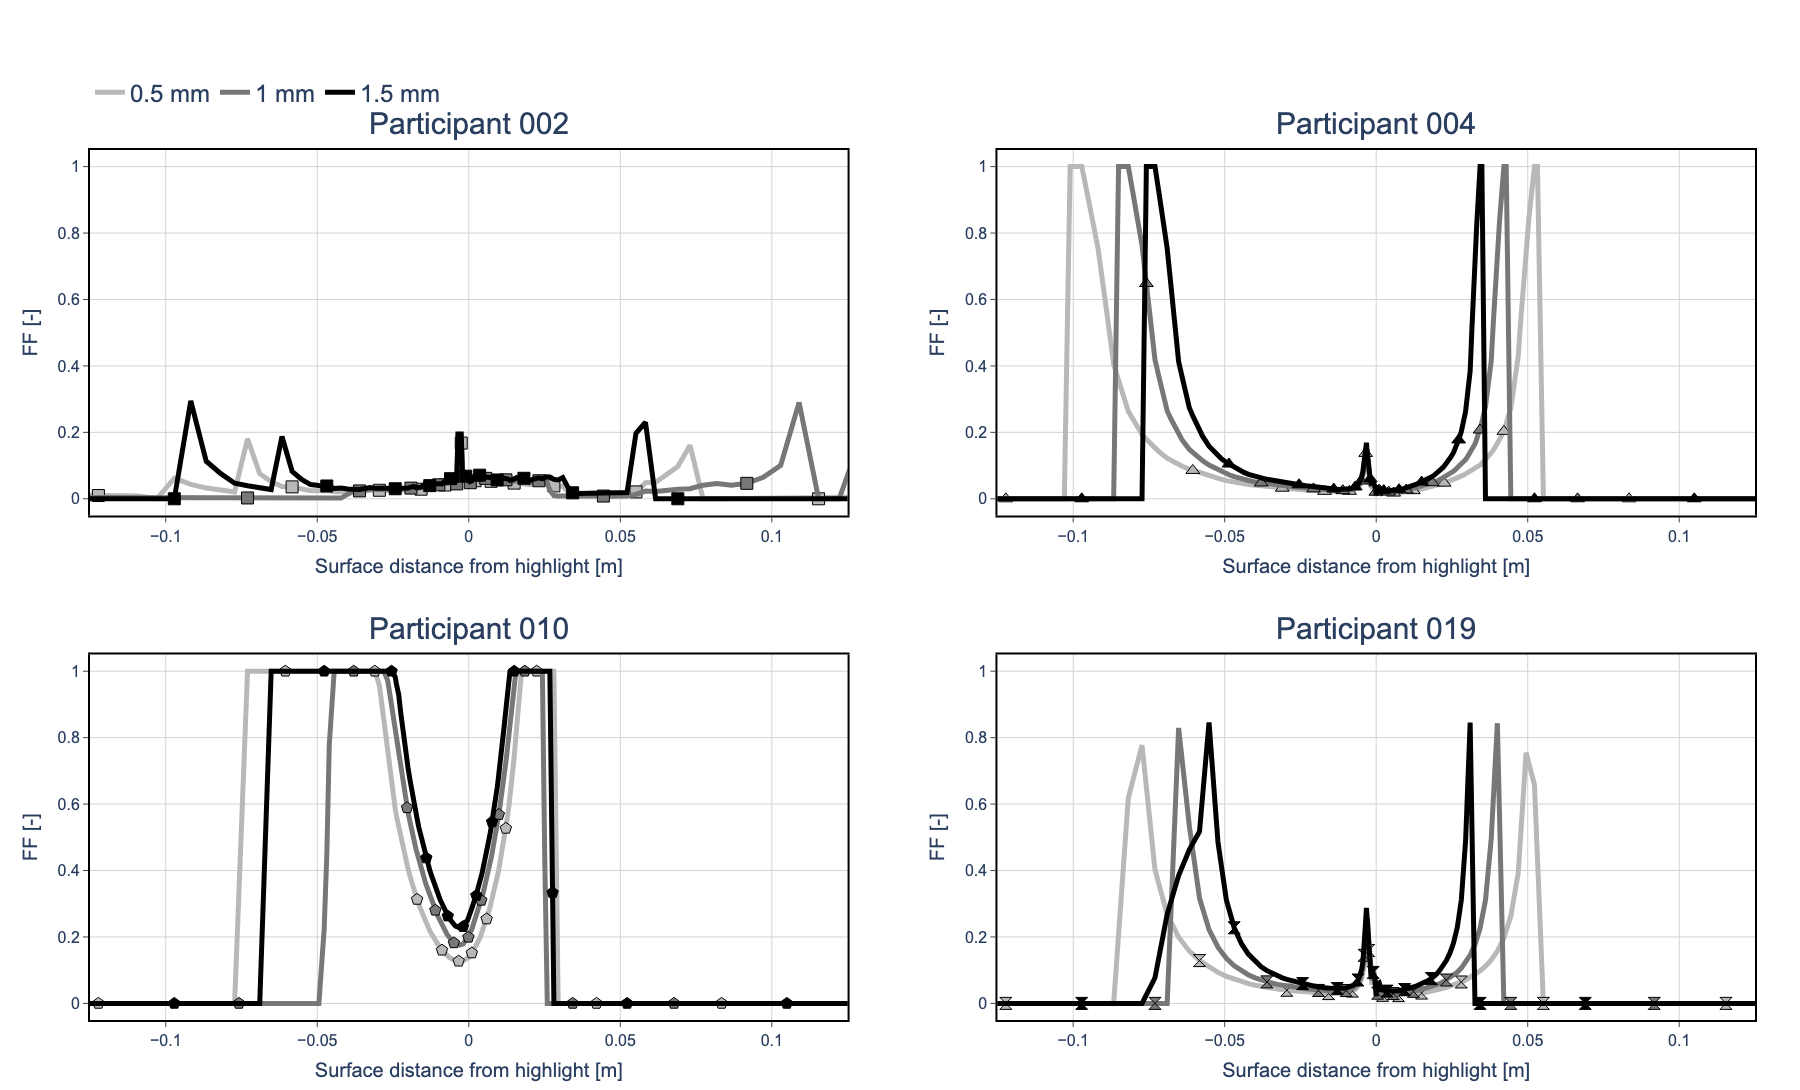
\includegraphics[width=0.7\textwidth]{FIGURES/SURF_TEMP_FF/tc_oneram6_L1_freezing_fraction_vs_s_slice_0p75_grouped_roughness_participants.png}

{\scriptsize\textbf{$y=0.75$ m -- Individual Participants}}

\end{frame}

% % ============================================================
% % ONERA M6 -- Mean Freezing Fraction
% % ============================================================

% \begin{frame}{\small ONERA M6 -- Mean Freezing Fraction Grid Convergence}
% \scriptsize

% % ------------------------------------------------------------
% % Middle slice -- 1 mm roughness
% % ------------------------------------------------------------
% \only<1>{
% \centering
% 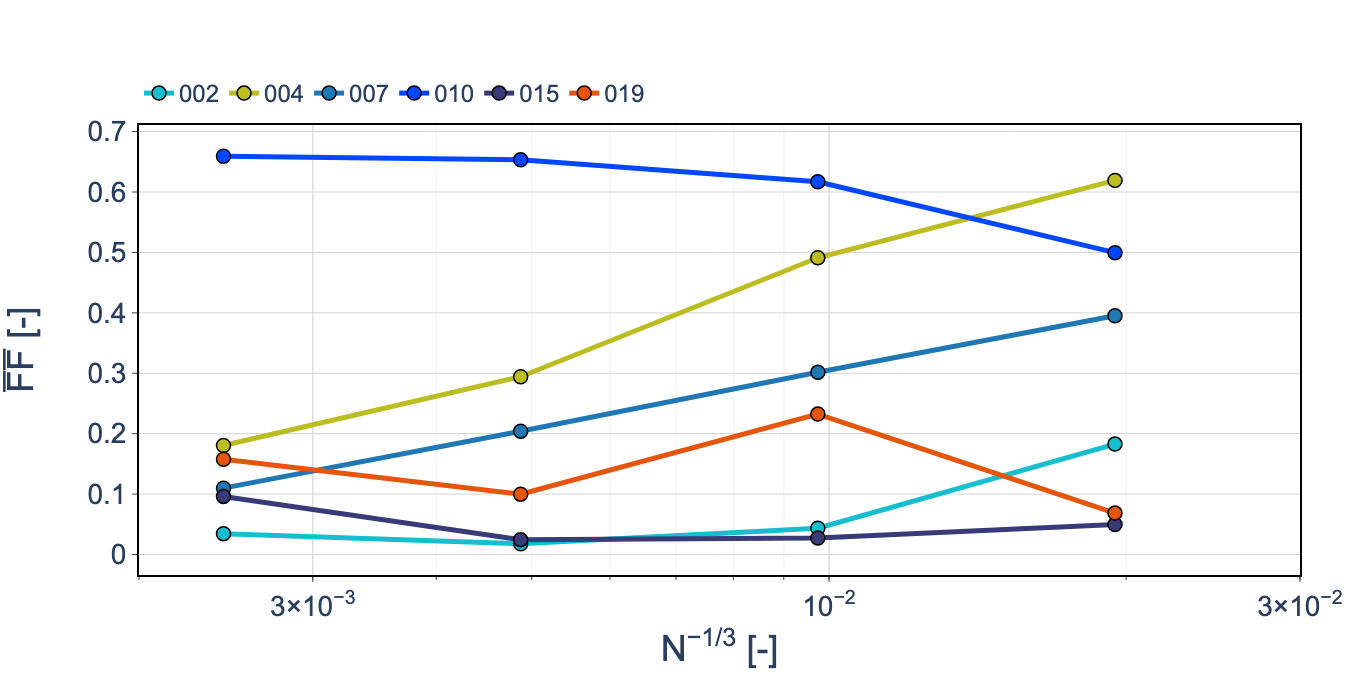
\includegraphics[width=0.5\textwidth]{FIGURES/SURF_TEMP_FF/tc_oneram6_mean_freezing_fraction_vs_n_slice_0p75_roughness_1mm.png}

% \vspace{0.05cm}

% \textbf{$y=0.75$ m}
% }

% % ------------------------------------------------------------
% % Inboard and outboard slices -- 1 mm roughness
% % ------------------------------------------------------------
% \only<2>{
% \begin{columns}[T,onlytextwidth]

% \begin{column}{0.50\textwidth}
%     \centering
%     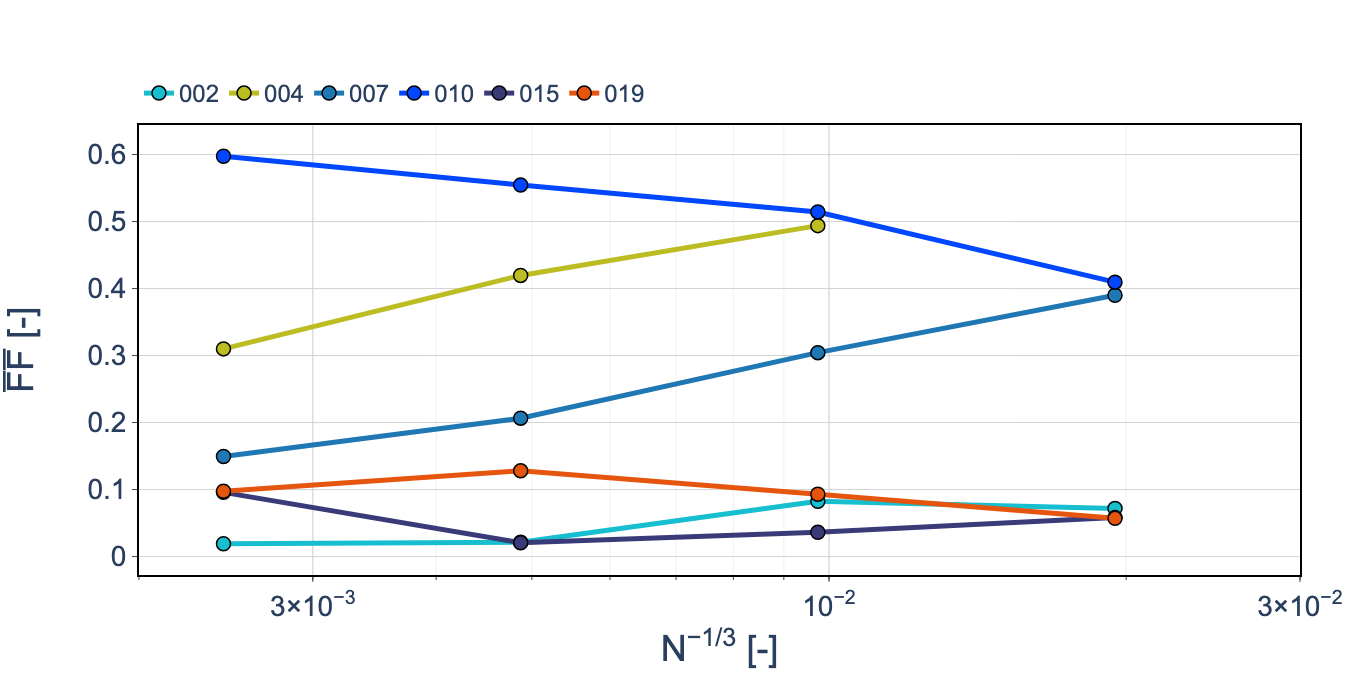
\includegraphics[width=0.94\textwidth]{FIGURES/SURF_TEMP_FF/tc_oneram6_mean_freezing_fraction_vs_n_slice_0p1_roughness_1mm.png}

%     \vspace{0.05cm}

%     \textbf{$y=0.10$ m}
% \end{column}

% \begin{column}{0.50\textwidth}
%     \centering
%     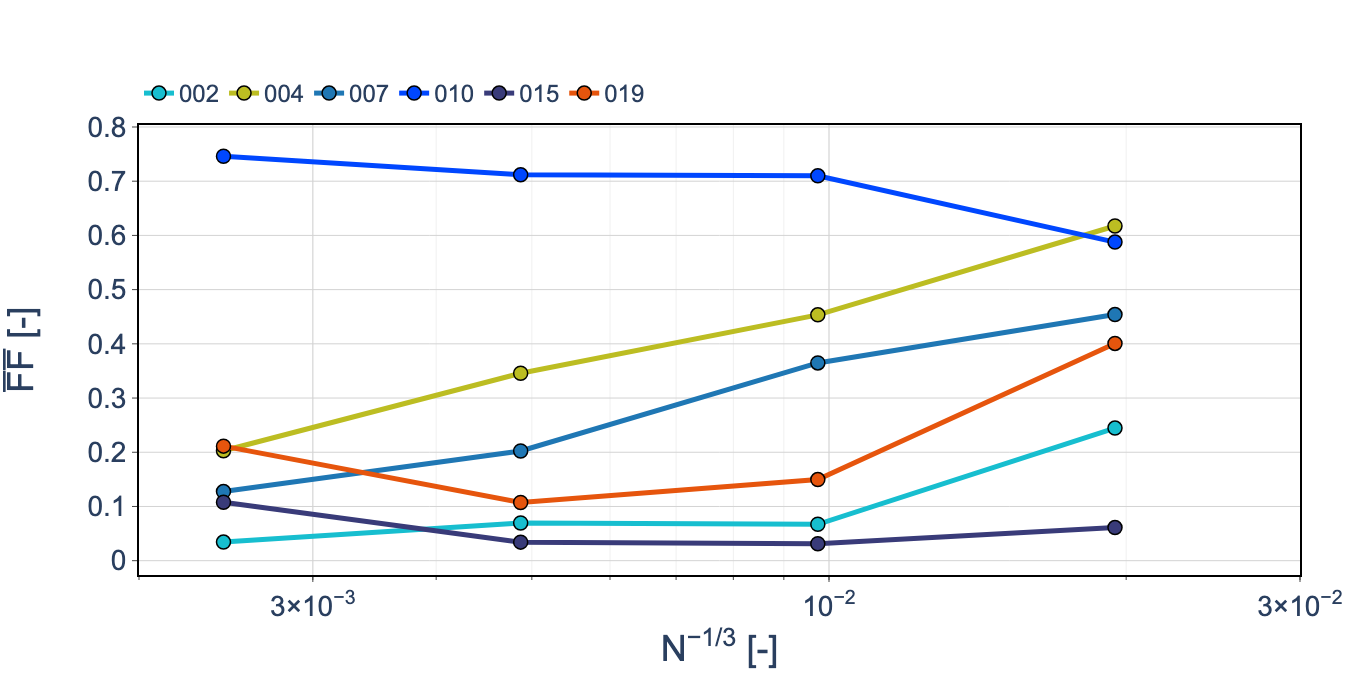
\includegraphics[width=0.94\textwidth]{FIGURES/SURF_TEMP_FF/tc_oneram6_mean_freezing_fraction_vs_n_slice_1p4_roughness_1mm.png}

%     \vspace{0.05cm}

%     \textbf{$y=1.40$ m}
% \end{column}

% \end{columns}
% }

% % ------------------------------------------------------------
% % Middle slice -- roughness sensitivity
% % ------------------------------------------------------------
% \only<3>{
% \centering
% 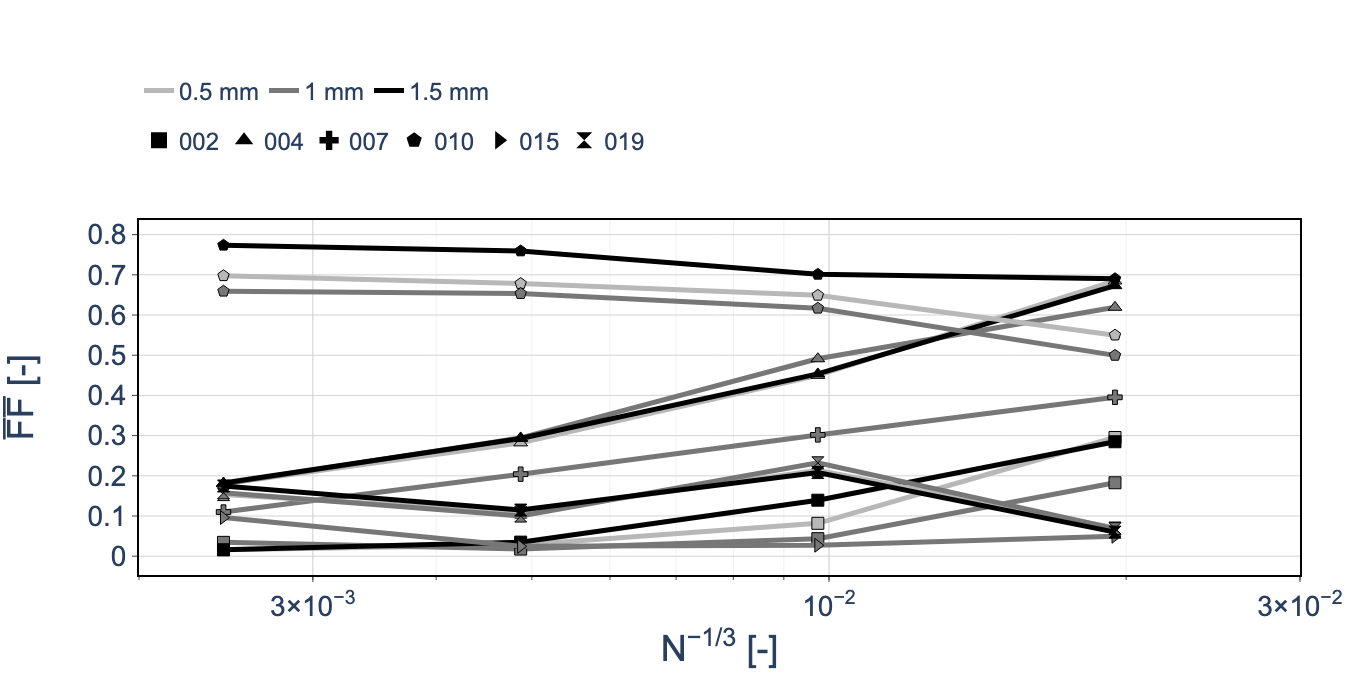
\includegraphics[width=0.5\textwidth]{FIGURES/SURF_TEMP_FF/tc_oneram6_mean_freezing_fraction_vs_n_slice_0p75_grouped_roughness.png}

% \vspace{0.05cm}

% \textbf{$y=0.75$ m- Roughness Sensitivity}
% }

% \vspace{0.10cm}

% \begin{block}{\scriptsize Observations}
% \begin{itemize}
%     \item<1-> Mean freezing fraction exhibits very large code-to-code variability, despite the comparatively close mean surface-temperature predictions for most submissions.
%     \item<1-> Grid sensitivity is submission-dependent, with some predictions remaining relatively stable while others vary substantially across the grid hierarchy.
%     \item<2-> Large code-to-code differences persist at the inboard and outboard spanwise stations.
%     \item<3-> Prescribed surface roughness introduces an additional systematic effect.
% \end{itemize}
% \end{block}

% \end{frame}

% % ============================================================
% % ONERA M6 -- Participant-Level Roughness Sensitivity
% % ============================================================

% \begin{frame}{\small ONERA M6 -- Participant-Level Freezing Fraction Roughness Sensitivity (L1)}
% \scriptsize
% \vspace{-0.2cm}
% \centering
% 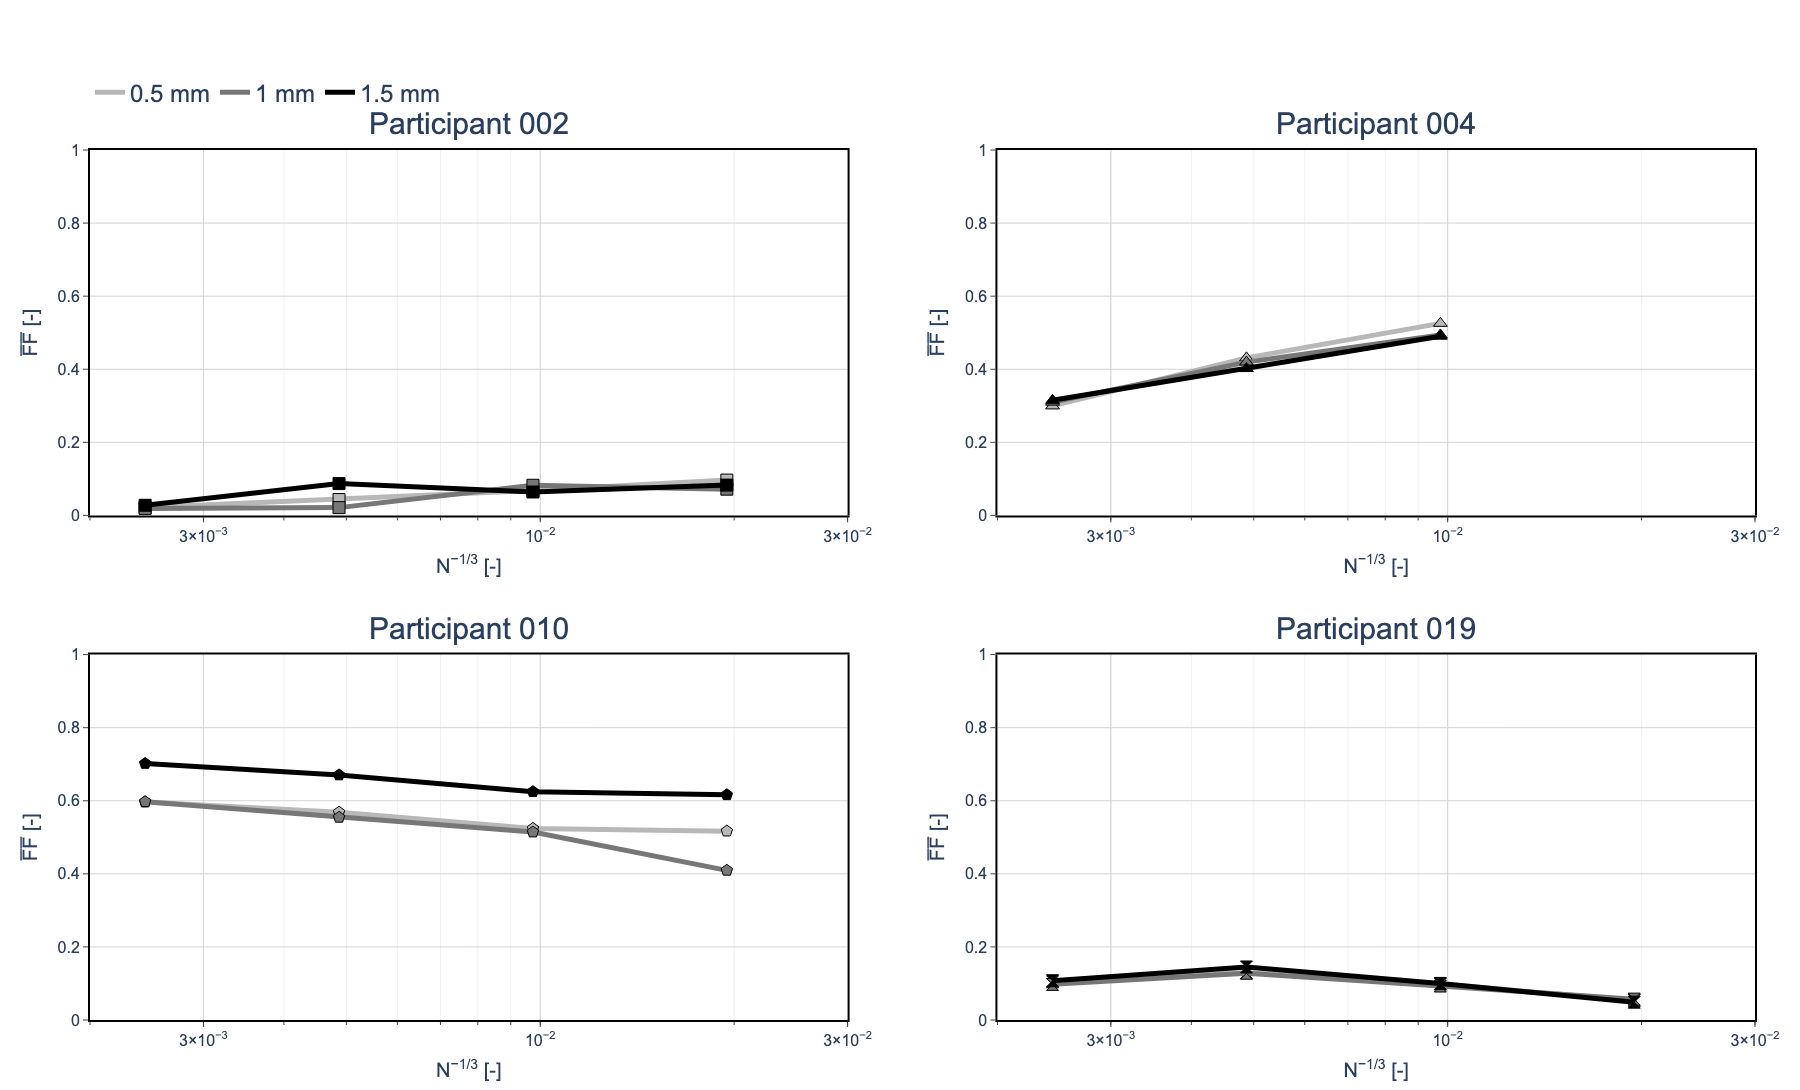
\includegraphics[width=0.8\textwidth]{FIGURES/SURF_TEMP_FF/tc_oneram6_mean_freezing_fraction_vs_n_slice_0p1_grouped_roughness_participants.png}

% \end{frame}

% ============================================================
% ONERA M6 -- Convective Heat Transfer & Thermodynamics Summary
% ============================================================

\begin{frame}{\small ONERA M6 -- Convective Heat Transfer \& Thermodynamics Summary}
\scriptsize

\begin{block}{\scriptsize Convective Heat Transfer}
\begin{itemize}
    \item Considerable code-to-code variability is observed in $HTC$, while reconstructed $T_{\mathrm{rec}}$ distributions remain closely aligned.
    \item Consequently, $Q_c'$ exhibits substantial code-to-code variability, with an L1 IQR of $83.9$ W/m at $y=0.75$ m.
\end{itemize}
\end{block}

\vspace{0.10cm}

\begin{block}{\scriptsize Surface Thermodynamics}
\begin{itemize}
    \item Mean surface temperature shows limited grid sensitivity and comparatively close agreement for most submissions.
    \item In contrast, freezing fraction exhibits larger code-to-code variability in both magnitude and spatial extent.
\end{itemize}
\end{block}

\vspace{0.10cm}

\begin{block}{\scriptsize Roughness Sensitivity}
\begin{itemize}
    \item Increasing roughness consistently increases $HTC$ and $|Q_c'|$.
    \item Mean surface temperature and freezing fraction exhibit code-dependent responses to roughness.
\end{itemize}
\end{block}

\vspace{0.10cm}

\begin{alertblock}{\scriptsize Thermodynamics Takeaway}
Despite consistent aerodynamic loading and $T_{\mathrm{rec}}$, substantial variability develops through the convective and freezing models, with the largest differences appearing in the predicted freezing regime.
\end{alertblock}

\end{frame}



